% Supplementary Methods and Figures for the DCN submission.
% Ported from the PNAS SI Appendix v9: acquisition, task descriptions, fMRI
% preprocessing and the registration detail stay here; tractography, RSA/
% clustering and the elastic net moved to the main-text Methods. Citations in
% this file are still plain text from the port -- convert to \citep on the
% final pass.
\documentclass[11pt]{article}
\usepackage[utf8]{inputenc}
\usepackage[T1]{fontenc}
\usepackage[round]{natbib}
\usepackage{graphicx}
\graphicspath{{../figures/manuscript/}{../figures/submitted/}{figures/manuscript/}{figures/submitted/}}
\usepackage{caption}
\usepackage[margin=2.5cm]{geometry}
\usepackage[hidelinks]{hyperref}

\title{Supplementary Materials\\ \large for ``The structural connectivity that
distinguishes the regions of adult prefrontal cortex is present in neonates''}
\author{Chiara Caldinelli \and Rhodri Cusack}
\date{}

\begin{document}
\maketitle

\section{Adult participants and acquisition}

Already preprocessed data from the The Human Connectome Project (HCP;
(https://www.humanconnectome.org/) was used for this study, and it was
obtained through Amazon Web Services. Here, data from a subgroup (n =
176) of the 1,200 healthy subject release with especially low head
motion was used. The participants were those identified by Ito and
colleagues in their exploratory cohort (Ito et al., 2017). The
participants comprised 99 females with a mean age of 29 years (range =
22--36 years). All subjects gave signed, informed consent and this study
was approved by the Washington University institutional review board.

\textbf{\emph{fMRI acquisition}}

Whole-brain multiband echo-planar imaging acquisitions were collected on
a 32-channel head coil on a modified 3T Siemens Skyra with TR = 720 ms,
TE = 33.1 ms, flip angle = 52o, Bandwidth = 2,290 Hz/Px, in-plane FOV =
208x180 mm, 72 slices, 2.0 mm isotropic voxels, and a multiband
acceleration factor of 8. Data for each subject was collected over the
span of two days. On the first day, anatomical scans were collected
(including T1-weighted and T2-weighted images acquired at 0.7 mm
isotropic voxels) followed by two resting-state fMRI scans (each lasting
14.4 minutes), and ending with a task fMRI component. The second day
consisted of a diffusion imaging scan, followed by a second set of two
resting-state fMRI scans (each lasting 14.4 minutes), and again ending
with a task fMRI session.

\textbf{\emph{Diffusion acquisition}}

High-quality diffusion-weighted MRI data were acquired using a 3T
Scanner Siemens Prisma. Images were acquired using a spin echo EPI
sequence with a multiband factor of 3, with a 210x180 field of view (RO
x PE), flip angle was 78 degrees, TR was 5520 ms, TE was 89.5 ms, 111
slices were acquired, each with a thickness of 1.25 mm, voxels were 1.25
mm isotropic, echo spacing was 0.78 ms, b-values were 1000, 2000, and
3000 s/mm2. Acquisition time was approximately 9 m and 50 s, 270
diffusion weighting directions, diffusion weighting consisted of 3
shells of b=1000, 2000, and 3000 s/mm2 interspersed with an
approximately equal number of acquisitions on each shell within each
run. The diffusion directions were obtained using a toolbox available
from Emmanuel Caruyer that returns uniformly distributed directions in
multiple q-space shells. The directions are optimized so that every
subset of the first M directions is also isotropic.

\section{Neonatal participants and acquisition}

Infant data included in this study is part of the second data release of
the The Developing Human Connectome Project (dHCP), comprising 558
neonates, with 490 fully usable sessions diffusion imaging data from 445
unique participants, 400 with a single session and 45 with two sessions.
Participants born preterm (less than 37 weeks of gestation, n=119) were
excluded. Participants included in this study were born at term, with a
gestational age ranging from 37 to 42 weeks. Of the 326 term-born
participants, usable tractography was obtained for 325, who form the
analysed sample: 175 males (mean gestational age 39.87 weeks, mean birth
weight 3.42 kg) and 150 females (mean gestational age 39.98 weeks, mean
birth weight 3.26 kg). One female participant was excluded for failed
diffusion processing. Infants were scanned while sleeping (without
sedation) at the Evelina Newborn Imaging Centre, St
Thomas\textquotesingle{} Hospital, London, UK. Ethical approval was
obtained from the UK Health Research Authority.

\textbf{\emph{Diffusion acquisition}}

Diffusion weighted MRI (DW-MRI) images were obtained with a 3T Philips
Achieva scanner using a customized 32-channel neonatal head coil. Images
were acquired using an optimized multi-shell HARDI sequence which varied
the number of directions on four shells (b = 0, b = 400, b = 1000, b =
2600) designed to optimize the white and grey matter contrast in
neonates. All four phase encoding directions were used and the voxel
size was 1.5 mm isotropic. The scan lasted approximately 20 minutes. If
the neonate woke up during the scan and subsequently settled, scan was
restarted to overlap with the previous acquisition. More details
regarding the diffusion acquisition can be found in (Bastiani et al.,
2019).

\textbf{\emph{Diffusion preprocessing}}

Data used in this study was already preprocessed, and more information
can be found in {[}Bastiani et al., 2019{]}. Susceptibility induced
distortions were corrected using estimation from the four PE directions
acquired. Images were corrected for Eddy\textquotesingle s currents and
motion using FSL\textquotesingle s EDDY. Outlier slices were detected,
replaced and slice-to-slice motion correction was performed. A super
resolution algorithm was applied to resample the thicker slice spacing
(3 mm) onto the isotropic grid (1.5 mm).

\section{fMRI tasks}

The tasks were: working memory, motor function, language processing,
social cognition, relational processing, emotion processing and
incentive processing. The tasks were extensively described in (Barch et
al., 2013), a brief description is given below.

\textbf{\emph{Working memory}}

There were 2 runs, each showing 4 categories: faces, places, tools and
body parts. Half of the run was used for a 0-back task and the other
half for a 2-back task. In the 0-back task, a target cue was presented
at the start of each block, and the participant had to press a button to
any presentation of that stimulus during the block. In the 2-back task,
participants had to respond to any item that was the same as the one 2
before. A cue was presented for 2.5 s, indicating the task type at the
start of the block. There were 8 blocks for each of the 2 runs, (10
trials of 2.5 s each, for a total of 25 s) and 4 fixation blocks (15 s
each). For each trial, the stimulus was presented for 2 s, followed by
500 ms during which the participant needed to answer. Each block
contained 10 trials, of which 2 were targets, and 2--3 were non-target
lures (e.g., repeated items in the wrong n-back position, for example
3-back). The four categories of stimuli were chosen because previous
studies showed that they reliably activate different cortical regions
across participants (Downing et al., 2006; Fox et al., 2009; J. C.
Taylor et al., 2007).

\textbf{\emph{Motor}}

This task was adapted from the one developed by Buckner and colleagues
(Buckner et al., 2011). There were 2 runs in total. A visual cue
instructed participants to tap their left or right fingers, squeeze
their left or right toes, or move their tongue. The cue was lasting for
3 s and each block of a movement type lasted for 12 s (10 movements).
For each run there were 13 blocks, with 2 of tongue movements, 4 of hand
movements (2 right and 2 left), 4 of foot movements (2 right and 2 left)
and three 15 s fixation blocks per run. This task was previously shown
to reliably identify specific activations in individual subjects (Thomas
Yeo et al., 2011).

\textbf{\emph{Language processing}}

This task was developed by (Binder et al., 2011) and consisted in two
runs that each interleaved 4 blocks of a story task and 4 blocks of a
mathematical task. The story blocks were a brief (5-9 sentences)
auditory story adapted from Aesop\textquotesingle s fables, followed by
a 2-alternative forced-choice question asking the participants about the
topic of the story. The example provided in the original Binder paper
(p.~1466) is "For example, after a story about an eagle that saves a man
who had done him a favor, participants were asked, \textquotesingle That
was about revenge or reciprocity?\textquotesingle". During the
mathematical task, the subjects were asked to complete addition and
subtraction problems. One example of a question is: "Fourteen plus
twelve"; followed by "equals" and then two choices: "twenty-nine or
twenty-six". The mathematics blocks were included because they provided
a comparison task that was attentionally demanding, similar in auditory
and phonological input, and unlikely to generate activation of anterior
temporal lobe regions involved in semantic processing, though likely to
engage numerosity related processing in the parietal cortex (Binder et
al., 2011). The blocks did not have the same length (average was 30 s)
but the mathematical task was matching the length of the story task
blocks, with several additional mathematics trials at the end of the
task to complete the 3.8 min run as needed. The mathematical task was
adaptive to maintain a similar level of difficulty across the
participants. For more details on the task, see Binder et al.~(2011).

\textbf{\emph{Social cognition (theory of mind)}}

A series of video clips was previously shown to be a reliable measure of
social cognition, generating robust task related activation in brain
regions associated with social cognition across subjects (Castelli,
2002; Castelli et al., 2000; Wheatley, T., 2007; White et al., 2011).
For this task, a shortened version of the original clips was used (20 s
instead of the original 40 s). A pilot study confirmed that the shorter
videos elicited similar responses to the longer videos. Each video clip
was showing objects (squares, circles, triangles; Abell et al., 2000)
either interacting, or moving randomly. After each video clip, the
participants had to choose between 3 answers: \textquotesingle the
objects interacted socially between each other\textquotesingle,
\textquotesingle Not Sure\textquotesingle, or \textquotesingle No
interaction\textquotesingle. Each of the two task runs had 5 video
blocks (2 Mental and 3 Random in one run, 3 Mental and 2 Random in the
other run) and 5 fixation blocks (15 s each).

\textbf{\emph{Relational processing}}

This task was adapted from a task published in (Smith et al., 2007), who
used it as a localizer for the anterior prefrontal cortex in individual
subjects. There, stimuli were 6 shapes filled with 6 different textures.
In the relational processing condition, the participants needed to
choose which one of the two pairs of objects presented at the bottom of
the screen was matching a pair shown at the top of the screen. First,
they only needed to decide if the two top objects had different shapes
or textures, then, if the two bottom objects also differed similarly. In
the control matching condition, the participants were shown two objects
at the top of the screen and one object at the bottom of the screen, and
a word in the middle of the screen (either "shape" or "texture"). They
were told to decide whether the bottom object matched either of the top
two objects on that dimension (e.g., if the word is "shape", is the
bottom object the same shape as either of the top two objects). In the
relational processing condition, the stimuli were presented for 3.5 s,
with an ITI of 0.5 s, and there were 4 trials per block. In the matching
condition, stimuli were presented for 2.8 s, with an ITI of 0.4 s, and 5
trials per block. Both blocks were 18 s long, and there were 3 blocks of
each type (relational processing and matching), plus 3 fixation blocks
lasting 16 s each.

\textbf{\emph{Emotion processing}}

This is an adapted version of a task published by Hariri and colleagues
that was shown to be a functional localizer (Hariri et al., 2006). The
task is organized in blocks. For each block the participant needed to
decide which one of the two faces at the bottom of the screen was
matching one face shown at the top, or which one of the two shapes was
matching the shape at the top. The faces were either angry or fearful.
Every block was composed of 6 trials of either shapes or faces. Every
stimulus was shown for 2 s and ITI was 1 s. A cue lasting 3 s was shown
before the block started and it was indicating if it was a shape of face
block. There were in total 3 faces and 3 shapes blocks.

\textbf{\emph{Incentive processing}}

This task was adapted from the {[}Delgado et al.~(2000){]}, and was
chosen for its ability to activate reward regions in a way that is
robust and reliable across subjects (Delgado et al., 2000, Forbes et
al., 2009, May et al., 2004, Tricomi et al., 2004). Participants need to
play a card game where they are asked to guess the number on a mystery
card (represented by a "?") in order to win or lose money. They are told
that potential card numbers range from 1 to 9 and to indicate if they
think the mystery card number is more or less than 5 by pressing one of
two buttons on the response box. Feedback is the number on the card
(generated by the program as a function of whether the trial was a
reward, loss or neutral trial) and either: 1) a green up arrow with
"\$1" for reward trials, 2) a red down arrow next to − \$0.50 for loss
trials; or 3) the number 5 and a gray double headed arrow for neutral
trials. The "?" is presented for up to 1.5 s (if the participant
responds before 1.5 s, a fixation cross is displayed for the remaining
time), following by feedback for 1.0 s. There is a 1.0 s ITI with a "+"
presented on the screen. The task is presented in blocks of 8 trials
that are either mostly reward (6 reward trials pseudo randomly
interleaved with either 1 neutral and 1 loss trial, 2 neutral trials, or
2 loss trials) or mostly loss (6 loss trials interleaved with either 1
neutral and 1 reward trial, 2 neutral trials, or 2 reward trials). In
each of the two runs, there are 2 mostly reward and 2 mostly loss
blocks, interleaved with 4 fixation blocks (15 s each). All the
participants are provided with money as a result of completing the task,
though it is a standard amount across subjects.

\section{fMRI preprocessing and modelling}

The preprocessed data from the HCP pipeline were used in this study. A
summary is given below, but for a detailed description of the analysis
see {[}Glasser et al.~2013{]}. FSL topup (Andersson et al., 2003) and
FLIRT (Jenkinson et al., 2002; Jenkinson \& Smith, 2001) were used to
correct for the distortion of EPI images. The distorted EPI images with
opposite phase-encoding directions were registered to the distorted
gradient reference images. This registration is concatenated with the
topup-derived distortion field, producing a nonlinear transform that can
be used to undistort the fMRI images. The single-band reference image
was corrected for distortions using spline interpolation and was next
registered to the T1W image, by successively using FLIRT and FreeSurfer
(Greve \& Fischl, 2009). This ensured an accurate registration between
the structural and the fMRI data. The native volumes acquired in native
space were then transformed into MNI space using nonlinear warping with
a single spline interpolation, minimizing interpolation- induced
blurring. One of the volume parcellations resulting from the FreeSurfer
processing (Glasser, 2013), the wmparc, was binarized, dilated three
times and eroded twice to produce an accurate subject-specific brain
mask of the gray and white matter. This brain mask was then applied to
the volume registrations and normalized to a 4D whole brain.

Images were smoothed using an unconstrained 3D Gaussian kernel of FWHM =
4 mm. A general linear model (GLM) estimated time series for each run,
using FILM (Improved Linear Model with autocorrelation correction;
(Woolrich et al., 2001). Predictors were convolved with a double gamma
"canonical" hemodynamic response function (Glover et al., 2000) to
generate the main model regressors. Temporal derivative terms derived
from each predictor were used as confounds to compensate for
slice-timing differences and variability in the HRF delay across
regions. A Gaussian-weighted linear high pass filter with a cutoff of
200 s was also applied. Finally, the time series was prewhitened within
FILM (Woolrich et al., 2001) to correct for autocorrelations in the fMRI
data.

\textbf{\emph{GLM design and contrasts}}

Below it is a brief description of how the GLM model was designed, as
described in {[}Barch 2013{]}.

\textbf{\emph{Working memory}}

Eight predictors were included in the model for the Working Memory task,
one for each type of stimulus in each of the N-back conditions (i.e.,
2-Back Body, 0-Back Body, 2- Back Face and 0-Back Face). Each predictor
covered the period from the onset of the cue to the offset of the final
trial (27.5 s). Linear contrasts for these predictors were computed to
estimate effects of interest: 2-back (vs.~fixation), 0-back, 2-back vs.
0-back, each stimulus type versus baseline (e.g., Body vs.~fixation,
collapsing across memory load), and each stimulus type versus all
others.

\textbf{\emph{Incentive processing}}

Two predictors were included in the model for Incentive Processing ---
mostly reward and mostly loss blocks, each covering the duration of 8
trials (28 s). For this task, as with all other tasks, linear contrasts
of the parameter estimates were computed to compare each condition to
baseline and to each other.

\textbf{\emph{Motor}}

Five predictors were included in the Motor model --- right hand, left
hand, right foot, left foot, and tongue. Each predictor covered the
duration of 10 movement trials (12 s). The 3 s cue period prior to each
motor block was modeled separately to account for visual activation
related to the cue word presented on the screen at the beginning of each
block. Linear contrasts were computed to estimate activation for each
movement type versus baseline and versus all other movement types.

\textbf{\emph{Language and social cognition}}

The Story predictor covered the variable duration of a short story,
question, and response period (\textasciitilde30 s). The Math predictor
covered the duration of a set of math questions designed to roughly
match the duration of the story blocks. Two predictors were included in
the Social Cognition model --- Social and Random motion. Predictors were
based on the category of the video clip rather than the rating of the
individual. Each predictor covered the duration of a single video clip
(20 s).

\textbf{\emph{Relational processing}}

Relational processing and a control Matching condition. Each predictor
covered the duration of 18 s composed of four trials for the Relational
condition and five trials for the Matching condition.

\textbf{\emph{Emotion processing}}

Two predictors were included in the Emotional Processing task model.
Each predictor covered a 21 s duration composed of a cue and six trials.

\textbf{\emph{Contrasts used}}

All contrasts calculated against baseline were excluded from the
analysis, leaving 31. The full list of contrasts used for this analysis
is the following: WORKING\_MEM\_2BK\_BODY, WORKING\_MEM\_2BK\_FACE,
WORKING\_MEM\_2BK\_PLACE, WORKING\_MEM\_2BK\_TOOL,
WORKING\_MEM\_0BK\_BODY, WORKING\_MEM\_0BK\_FACE,
WORKING\_MEM\_0BK\_PLACE, WORKING\_MEM\_0BK\_TOOL, WORKING\_MEM\_2BK,
WORKING\_MEM\_0BK, WORKING\_MEM\_BODY, WORKING\_MEM\_FACE,
WORKING\_MEM\_PLACE, WORKING\_MEM\_TOOL, GAMBLING\_PUNISH,
GAMBLING\_REWARD, MOTOR\_CUE, MOTOR\_LF, MOTOR\_LH, MOTOR\_RF,
MOTOR\_RH, MOTOR\_T, MOTOR\_AVG, LANGUAGE\_MATH, LANGUAGE\_STORY,
SOCIAL\_RANDOM, SOCIAL\_TOM, RELATIONAL\_MATCH, RELATIONAL\_REL,
EMOTION\_FACES, EMOTION\_SHAPES. For more details of the contrasts and a
full description of the tasks, see the previous paragraph Stimuli and
{[}Barch et al., 2013{]}.

\section{Transformation of the adult parcellation into neonatal space}

A schematic summary of these transformations is shown in Fig. S1 and an
example of the results is shown in Fig. S2. To register the adult to the
infant space, we used the Advanced Normalization Tools (ANTs). ANTs has
proven performance in lifespan analyses of brain morphology (Tustison et
al., 2014) and function (Avants et al., 2014) in both adult (Tustison et
al., 2014) and pediatric brain data (Avants et al., 2014; Jain et al.,
2012; Lawson et al., 2013) including infants (Pineda et al., 2014). ANTs
employs both probabilistic tissue segmentation (via Atropos (Avants et
al., 2011) and machine learning methods based on expert labeled data
(via joint label fusion (H. Wang et al., 2011) in order to maximize
reliability and consistency of multiple modality image segmentation. We
used antsRegistrationSyN to register from an adult MNI-152 v.6
asymmetric T1-weighted template to the dHCP 40 weeks T1-weighted
template
(https://gin.g-node.org/BioMedIA/dhcp-volumetric-atlas-groupwise). We
identified two issues, discussed in more detail in Cabral et al (2022).
First, the cerebellum is substantially smaller in infants than adults
relative to the size of the cerebrum, which would cause misregistration.
We therefore masked the cerebellum during registration. Second, the
skull and scalp are thinner in infants. We therefore masked these. The
final registration can be seen in Cabral et al, (2022).

This transformation derived from the T1 was used to transform an adult
parcellation into the infant space. Specifically, the Glasser (Glasser
et al., 2016) parcellation label file was transformed into a volume
aligned with the MNI 152 v.6 template using the Workbench Connectome
software v1.5.0 (label to volume mapping command). From this volume
template, antsApplyTransforms was used to register this parcellation to
the dHCP 40 weeks template volume.

The dHCP release included the transformations from the dHCP 40 week
template in volumetric space to the individual infant\textquotesingle s
diffusion image space to the, which was applied to the parcellation
using FSL\textquotesingle s applywarp with nearest neighbor
interpolation. See Fig. S2 for an example of the transformation of the
adult DLPFC mask to the infant space (T1 template).

Tractography was run in native space . The resulting seed-to-target maps
were then transformed back to the adult MNI space in stages. First, they
were transformed from the individual\textquotesingle s native space to
the dHCP 40 week space using the dHCP releases\textquotesingle s
transformations with FSL\textquotesingle s applywarp. They were then
transformed from the dHCP 40 week space to the adult MNI space. Lastly,
workbench software v1.5.0 was used to sample the resulting volumes onto
a surface.

All the registration steps were manually checked for each infant to
ensure that the registration was successful.

\section{Subject-only cross-validation}

The main text evaluates every analysis under leave-one-region-out
cross-validation, so no prediction comes from a model that saw its own
territory. For comparison, this section reports the subject-only protocol
--- the convention in prior work --- in which models are trained on all
DLPFC vertices of the training participants and evaluated on the full map
of the held-out participant or neonate. Accuracies are uniformly higher
(adult own-map within-task $r$ 0.12--0.26; neonatal transfer 0.16--0.46;
task specificity 40 of 40 column-wise comparisons in both), the difference
being the within-region interpolation that the region-level protocol
removes. Under this protocol the raw motor transfer appears successful
($r = 0.24$ left, $0.16$ right); the main-text controls show that this
apparent success is carried by spatial smoothness, position and the
distance decay of tractography rather than by function-specific structure.
The leave-one-subject-out group-mean benchmark reported in the main text
(individual connectivity-based predictions never exceeding the group-average
map, 0 of 10 cells) was computed under this protocol.

\begin{figure}[p]
  \centering
  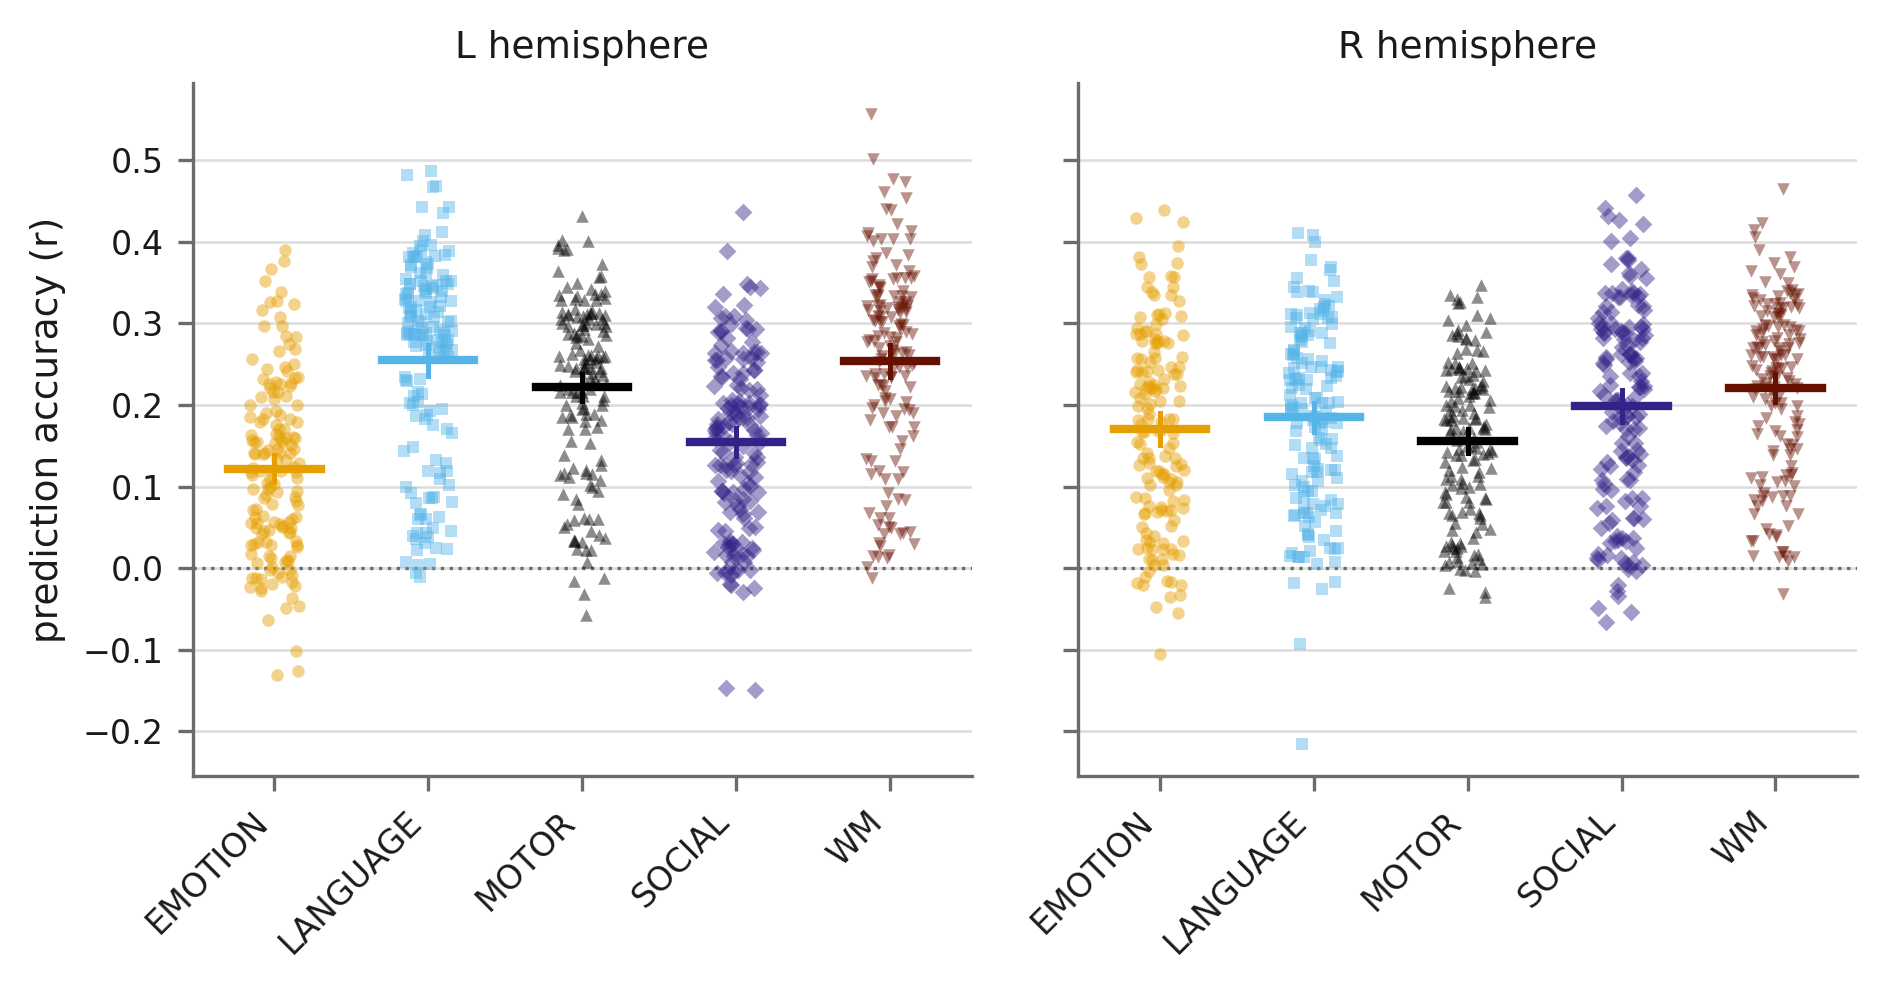
\includegraphics[width=.9\linewidth]{Fig2_adult_own_activation_accuracy.png}
  \caption*{\textbf{Fig.~S11.} Adult own-map prediction under subject-only
  cross-validation (conventions as in main-text Fig.~2A).}
\end{figure}

\begin{figure}[p]
  \centering
  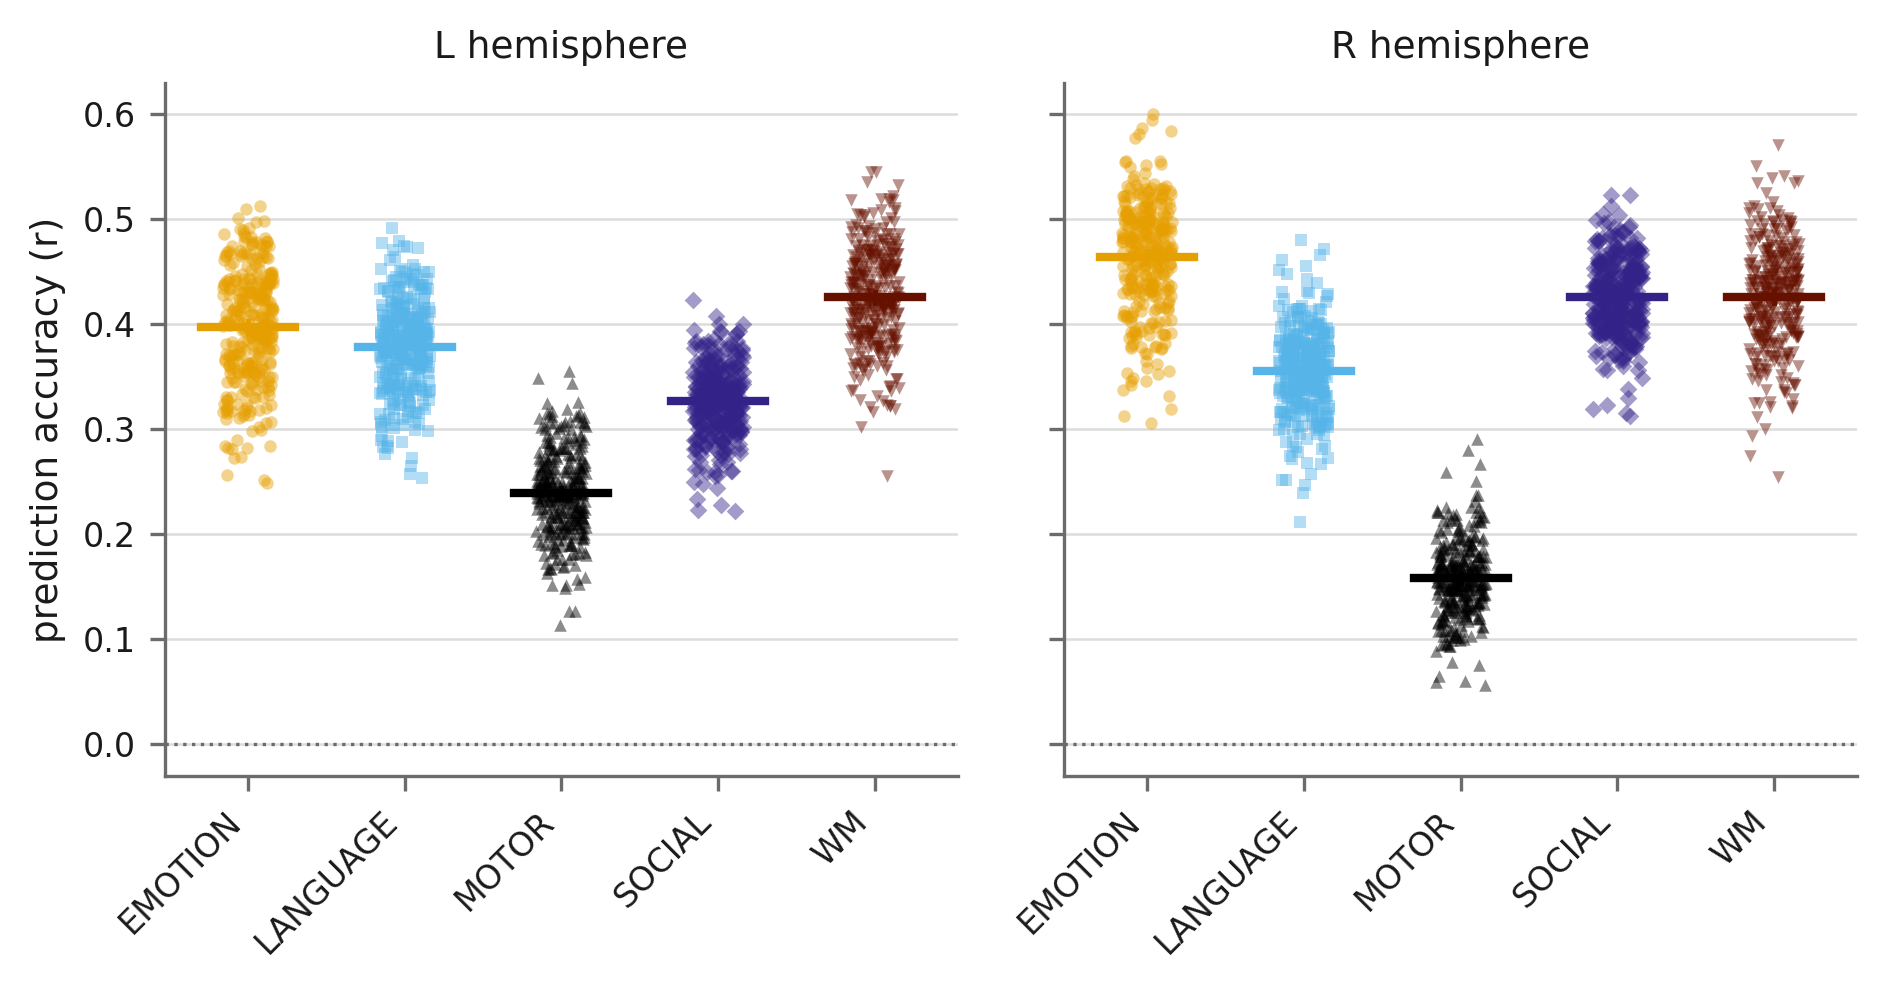
\includegraphics[width=.9\linewidth]{Fig3_neonatal_accuracy.png}
  \caption*{\textbf{Fig.~S12.} Neonatal transfer under subject-only
  cross-validation (conventions as in main-text Fig.~4A).}
\end{figure}

\begin{figure}[p]
  \centering
  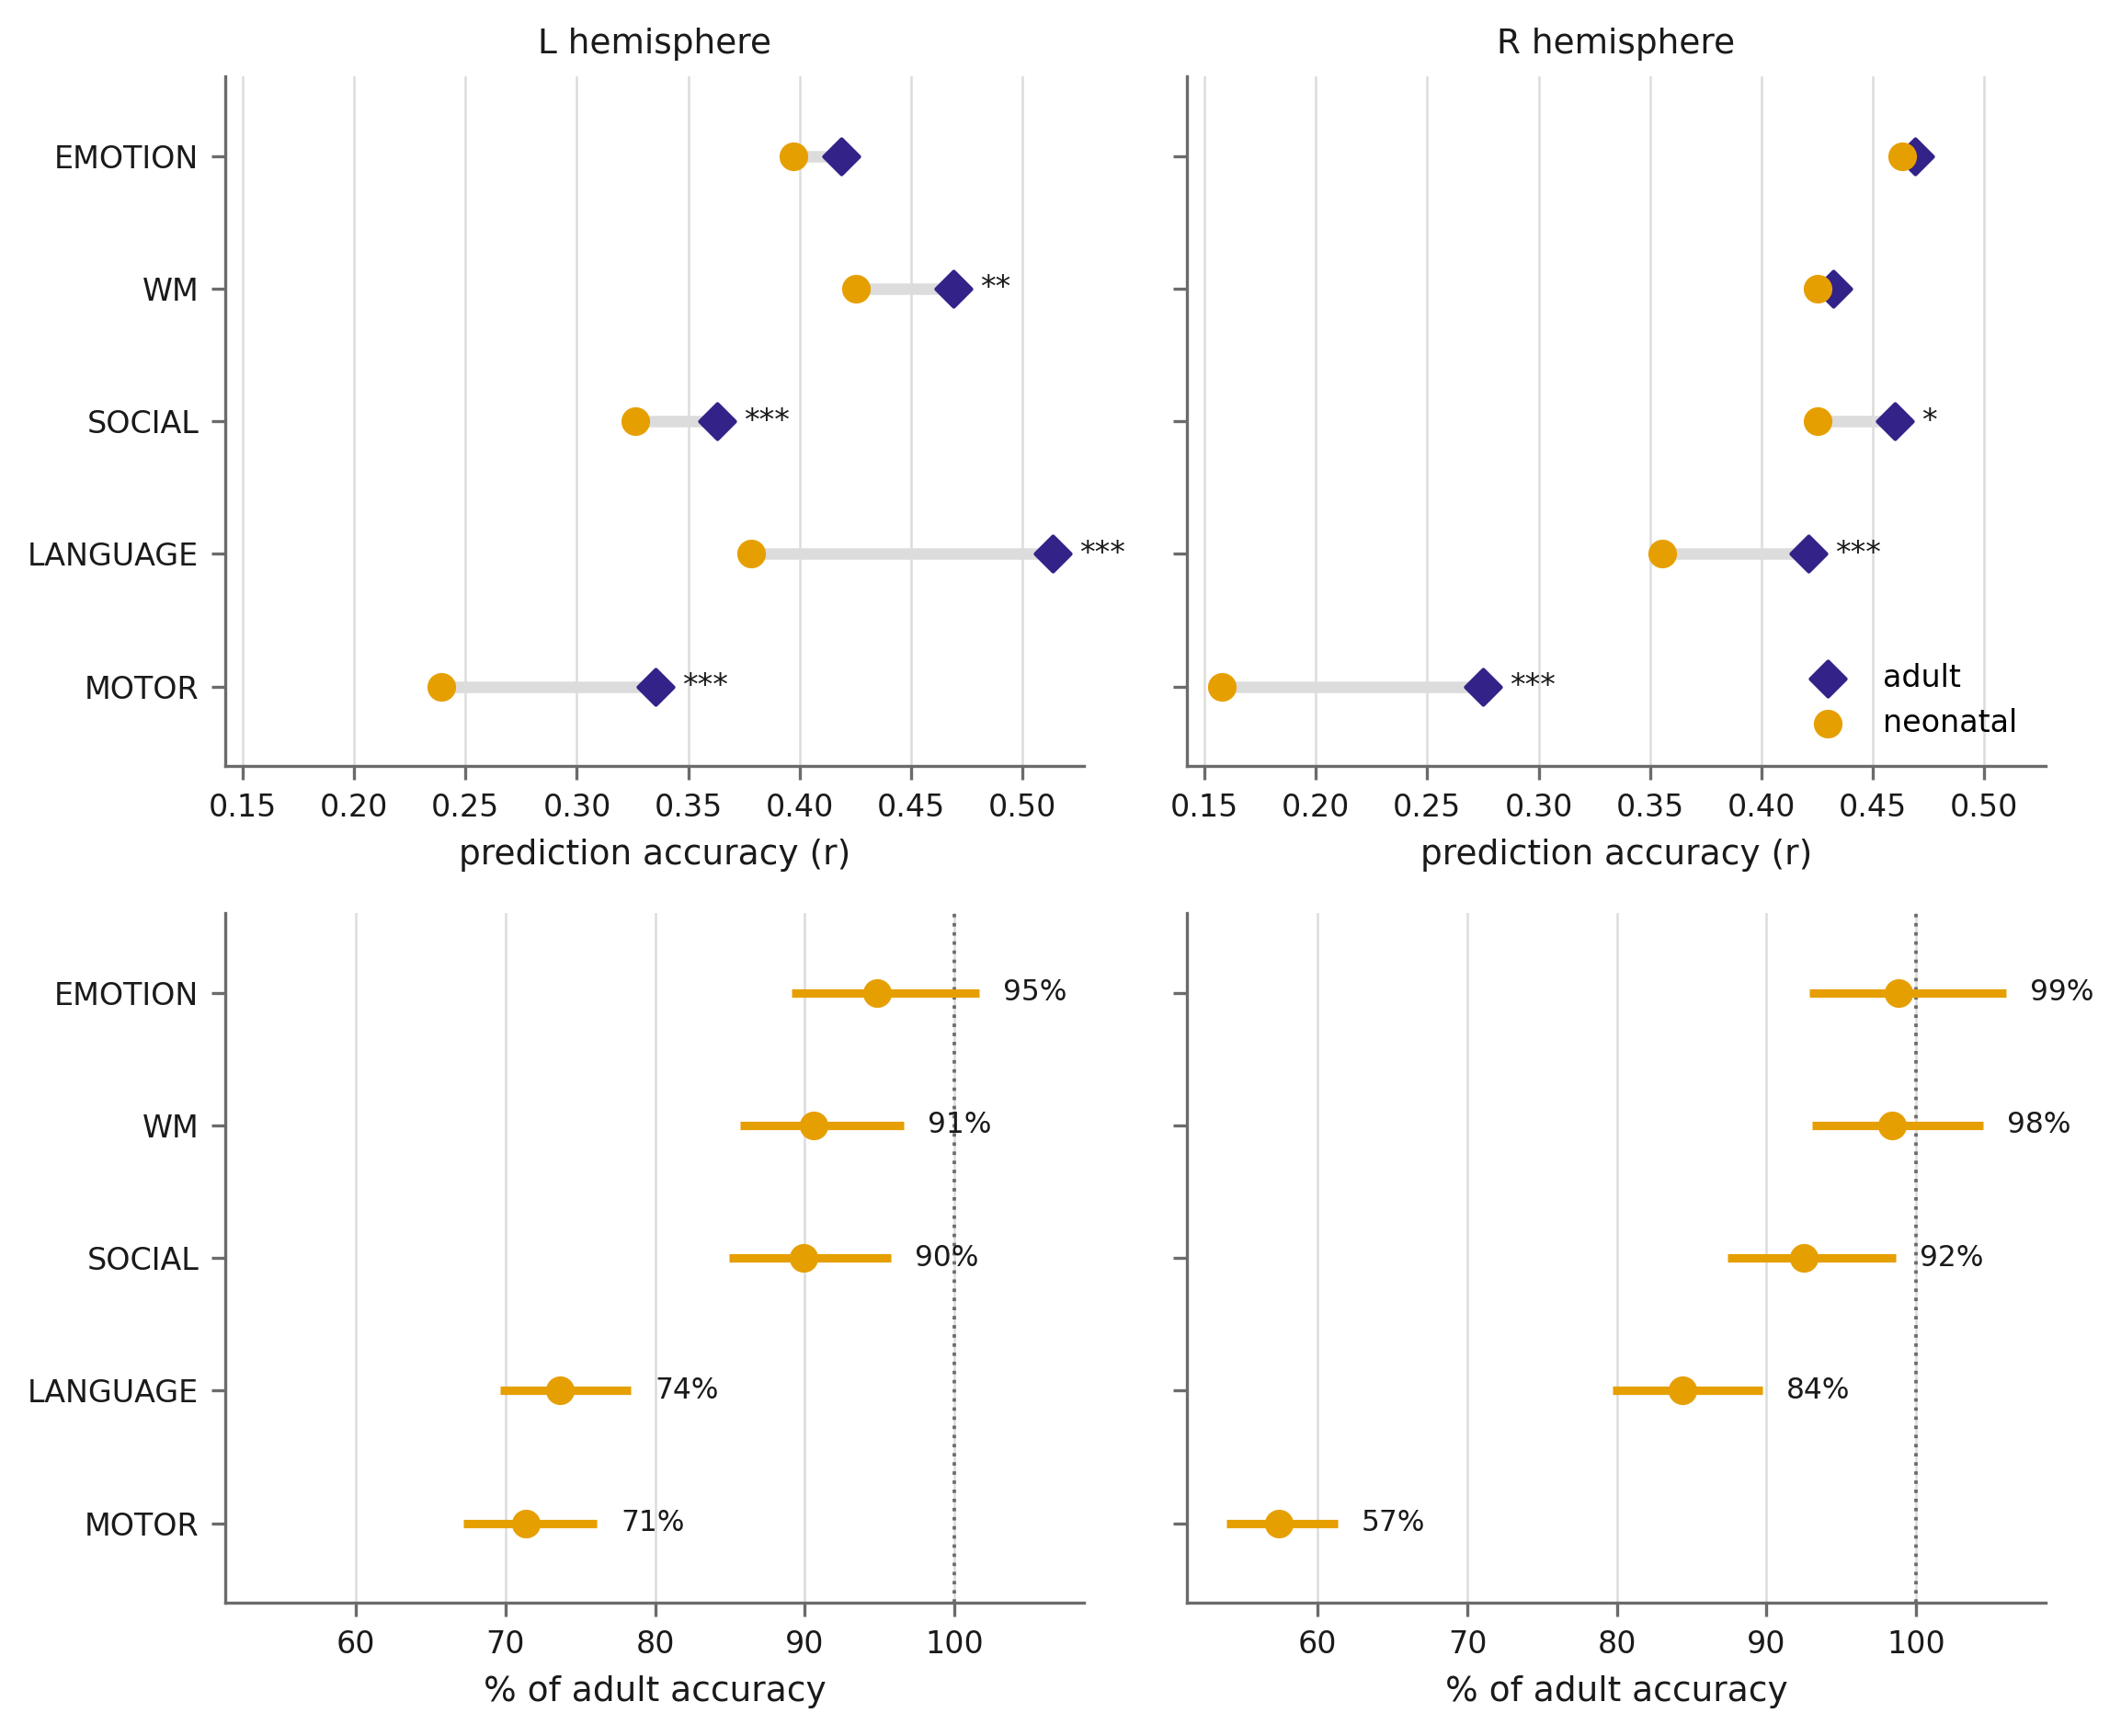
\includegraphics[width=.9\linewidth]{Fig4_neonate_vs_adult.png}
  \caption*{\textbf{Fig.~S13.} Neonatal accuracy as a proportion of adult
  accuracy under subject-only cross-validation (median 90\%, range
  57--99\%).}
\end{figure}

\section{Output-level spatial null}

Rotating a map defined only on the DLPFC displaces most vertices outside the
mask, with no values available to replace them. We therefore used
variogram-matched surrogate maps (Burt et al., 2020) generated within the
DLPFC mask, which preserve the spatial autocorrelation and the exact value
distribution of the observed map while destroying its correspondence with
the prediction. For each contrast and hemisphere we generated 1{,}000
surrogates of the adult group-average activation map, held each neonate's
predicted map fixed, and correlated it against every surrogate; the null
distribution is that of the across-neonate mean correlation, matching the
observed statistic. No model is refitted; the full-pipeline null, in which
models are refitted on spatially permuted training sets, is described in the
main text. $p_{\mathrm{spin}} = (k+1)/(n+1)$, where $k$ is the number of
surrogates reaching the observed value. Observed accuracy exceeded this null
for all ten task-by-hemisphere combinations ($p_{\mathrm{spin}} \le 0.002$,
Benjamini--Hochberg corrected); null distributions were centred near zero
(SD 0.055) and the smallest margin over the null mean was 0.160 (right
motor, 3.4 null SD). This null is approximately three times wider than a
permutation null that ignores spatial autocorrelation (SD 0.055 against
$\approx 0.02$): on a territory as compact as the DLPFC, two independently
generated smooth maps can correlate at $|r| \approx 0.7$ from shared spatial
structure alone, so raw correlations between DLPFC maps should not be
interpreted without a spatial null.

\section{Scan-age analysis}

Prediction accuracy from neonatal connectivity, averaged across the five
contrasts and both hemispheres, was regressed on postmenstrual age at scan,
gestational age at birth, and mean relative (volume-to-volume) motion from
the diffusion preprocessing ($n = 325$). Accuracy increased with age at scan
($\beta = 0.0024$ per week, $p = 0.040$) and with gestational age at birth
($\beta = 0.0043$ per week, $p = 0.007$), and decreased with motion
($\beta = -0.0037$ per mm, $p = 0.014$); $R^2 = 0.123$. Of the five
contrasts, only language showed an independent association with age at scan
after correction ($\beta = 0.0044$ per week, $p_{\mathrm{FDR}} = 0.0065$).
Two limits should be borne in mind. Age at scan and gestational age at birth
are correlated in a term-born cohort ($r = 0.71$), so their contributions
cannot be separated: the data show that accuracy rises with age, not which
age. And the effect is small --- 0.017 in $r$ across the full 7.3-week range
of scan ages, against a between-infant spread in accuracy of 0.28 to 0.42.
We therefore report these associations as exploratory.

\section{Supplementary Figures}

\begin{figure}[p]
  \centering
  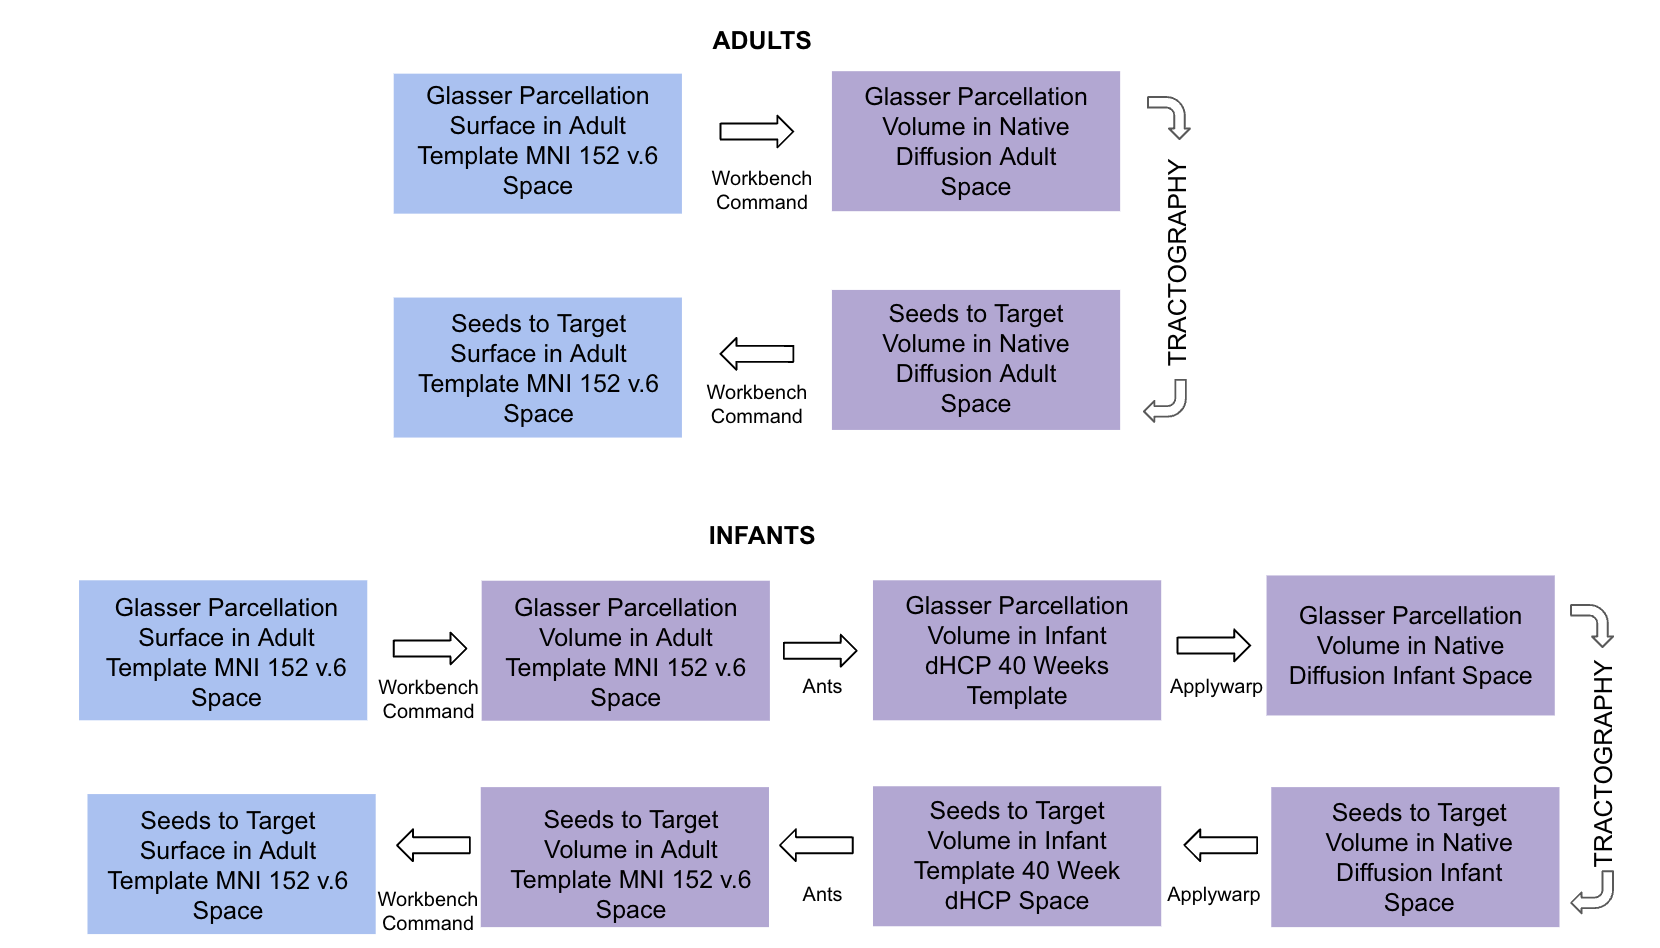
\includegraphics[width=.95\linewidth]{S1_registration_schematic.png}
  \caption*{\textbf{Fig.~S1.} Schematic of the transformations between adult
  and neonatal spaces. Upper row: adults. Lower row: infants, via the dHCP
  40-week template.}
\end{figure}

\begin{figure}[p]
  \centering
  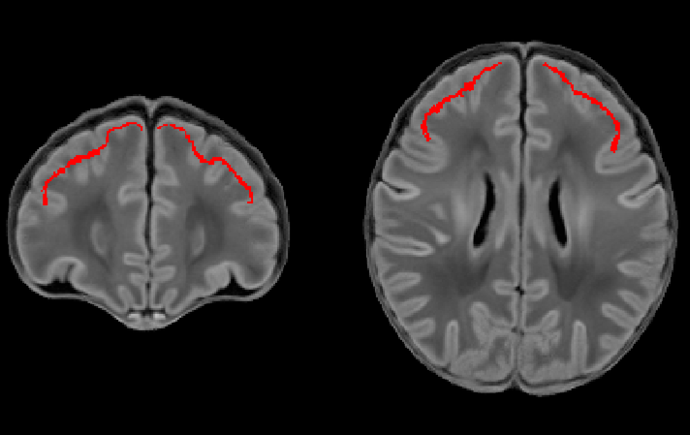
\includegraphics[width=.7\linewidth]{S2_registration_example.png}
  \caption*{\textbf{Fig.~S2.} Example transformation of the adult DLPFC mask
  (red) into an infant's space (left) alongside the adult template (right).}
\end{figure}

\begin{figure}[p]
  \centering
  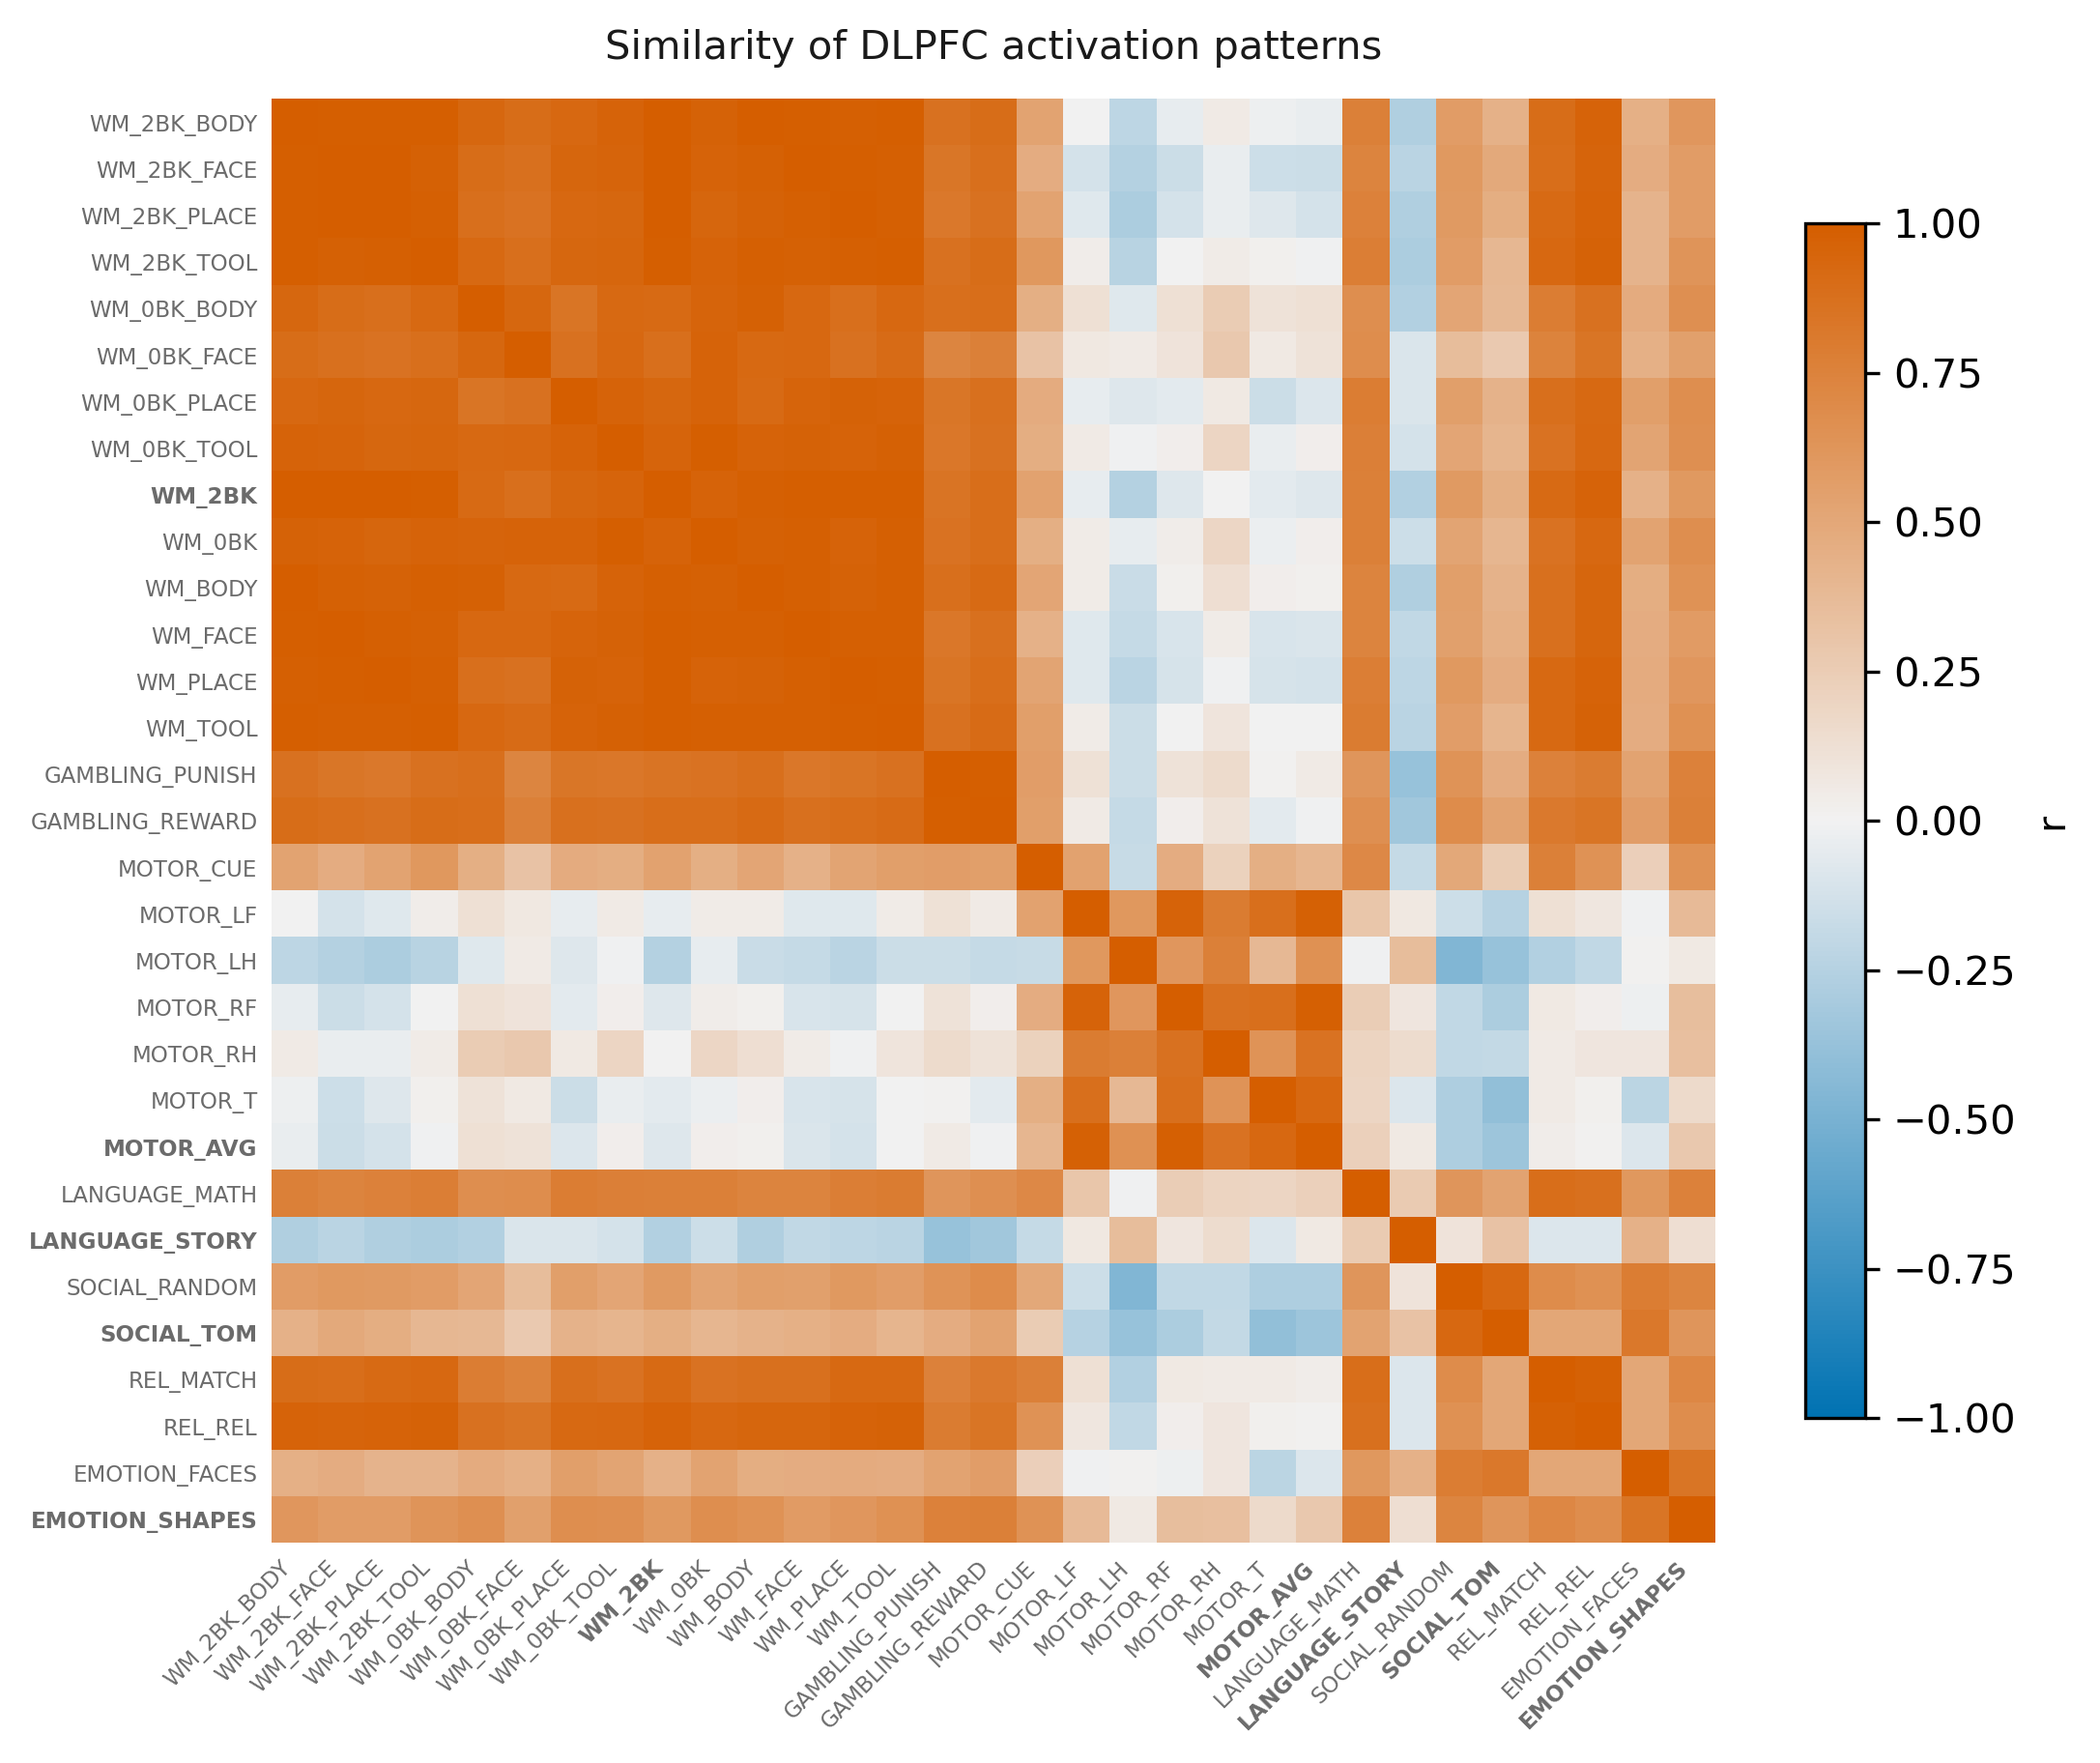
\includegraphics[width=.8\linewidth]{S3_similarity_matrix.png}
  \caption*{\textbf{Fig.~S3.} Similarity of the spatial patterns of the 31
  task contrasts across the 26 DLPFC parcels.}
\end{figure}

\begin{figure}[p]
  \centering
  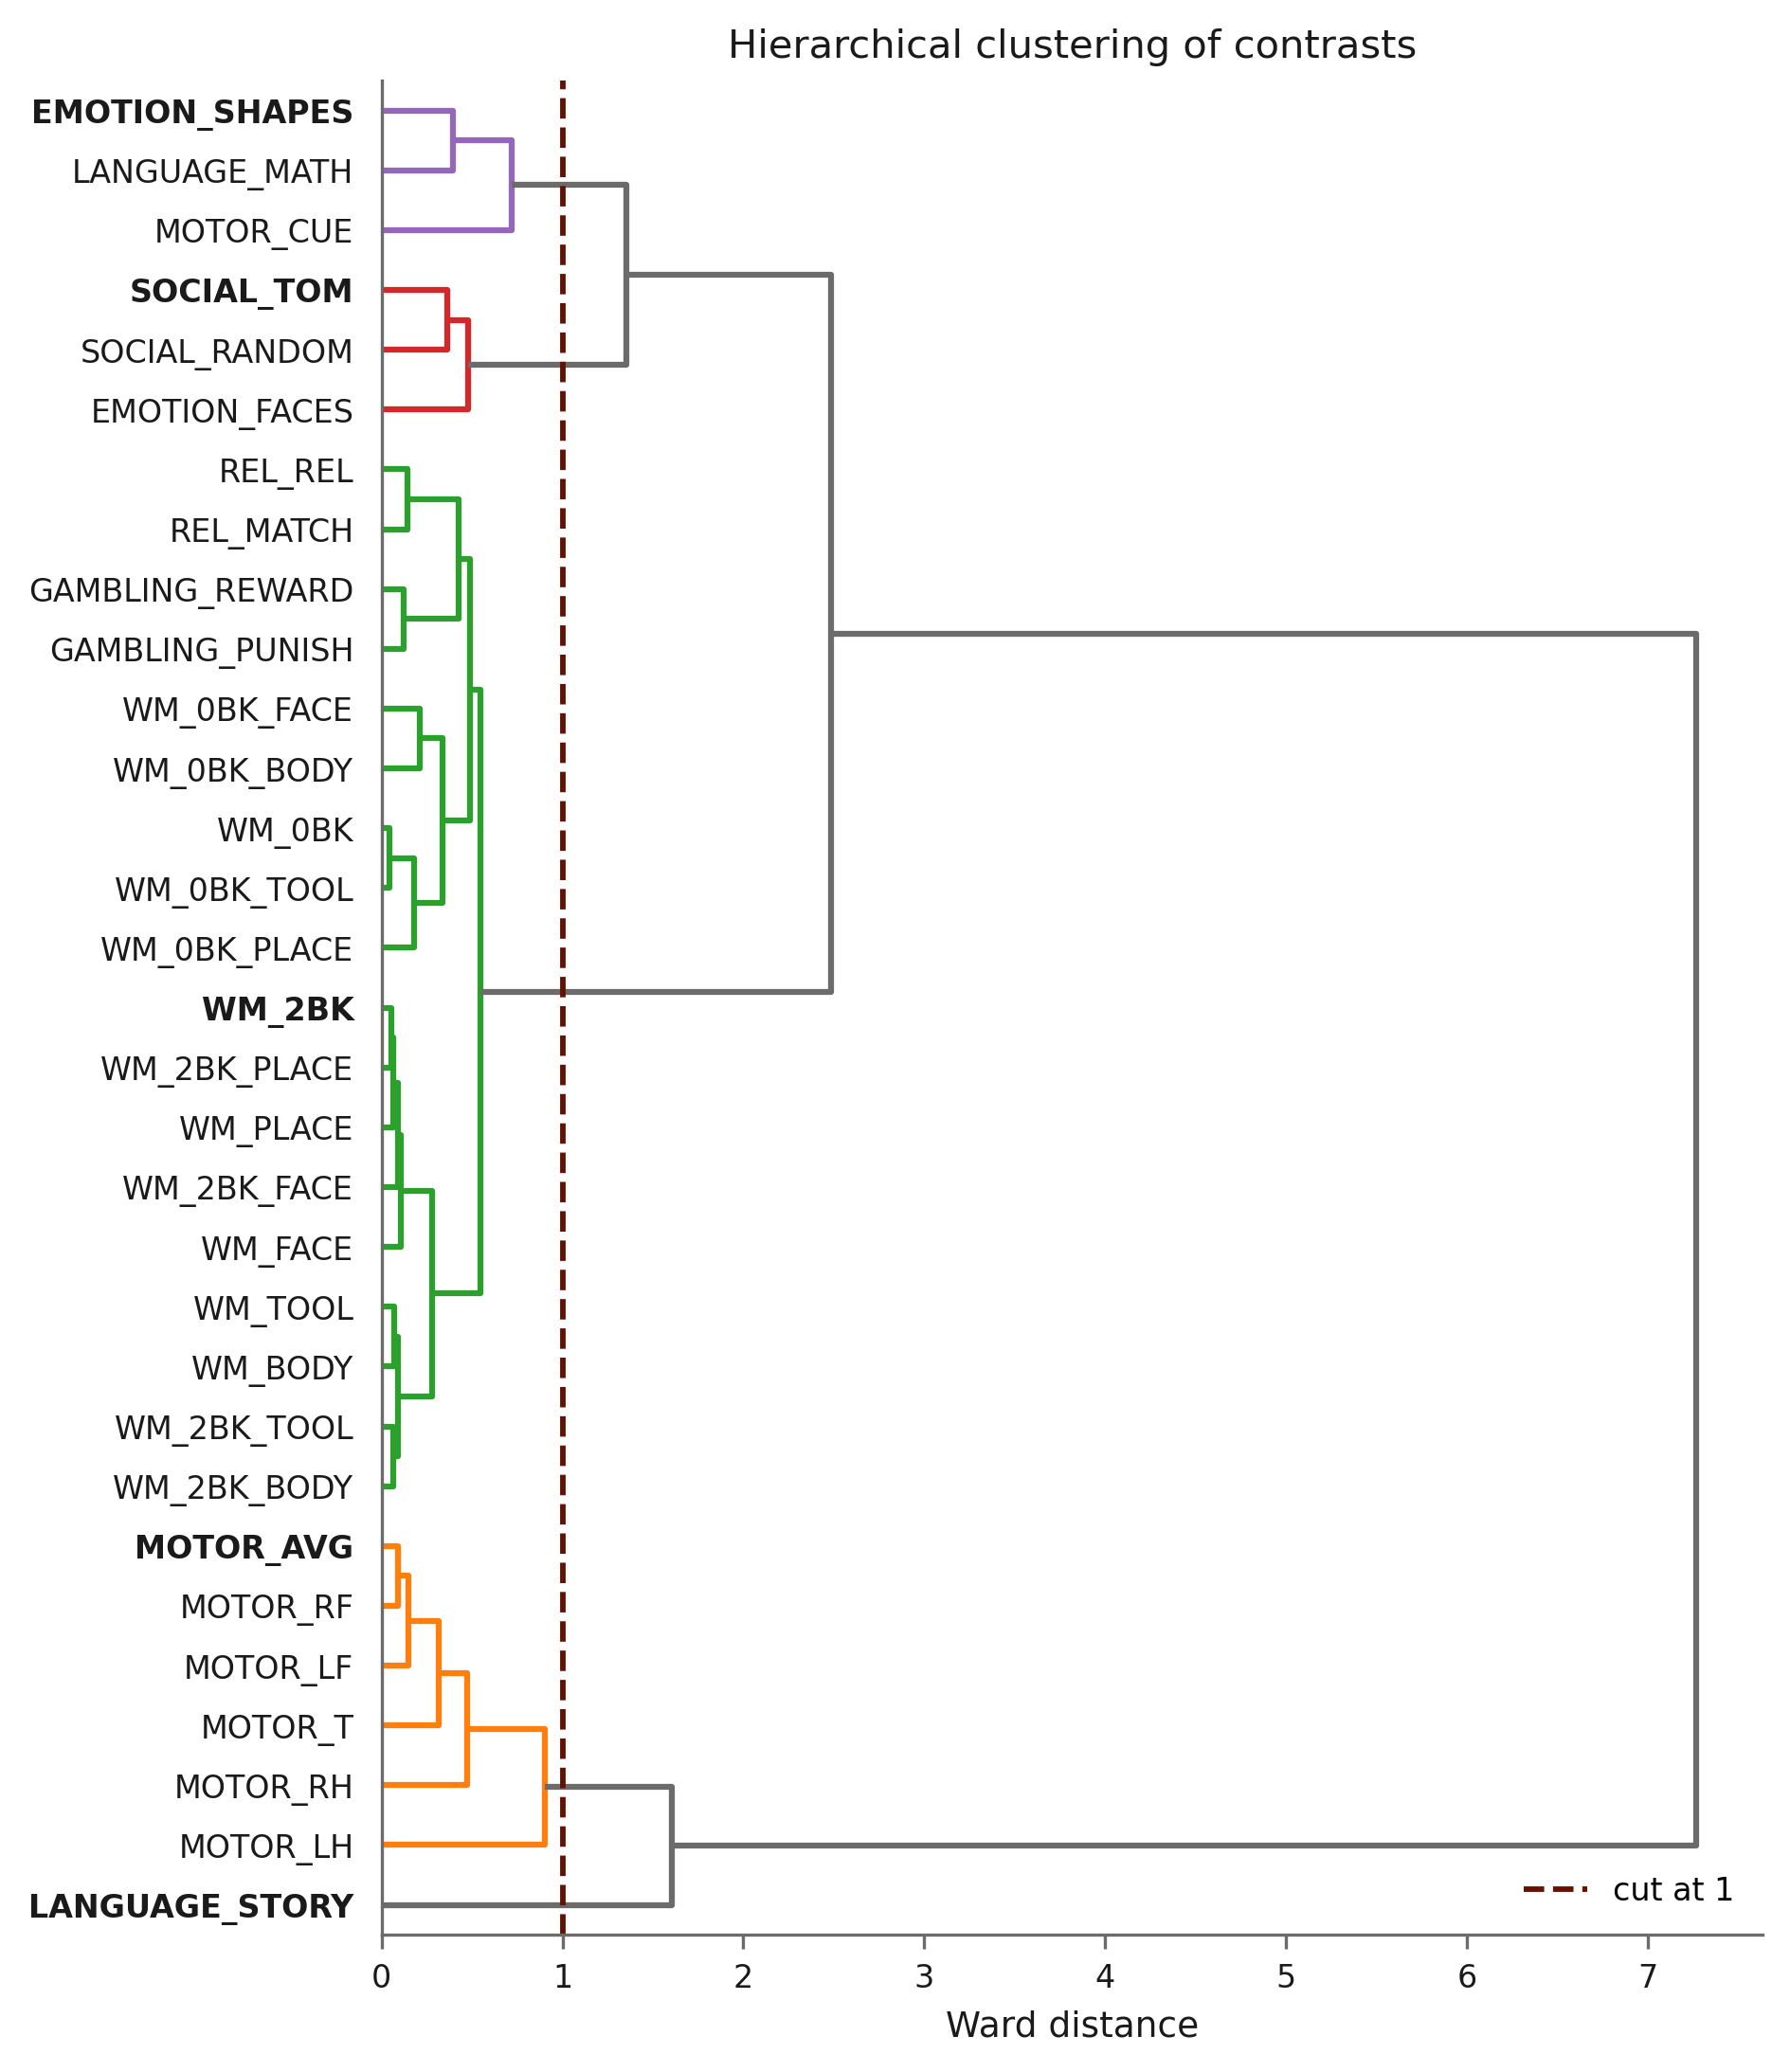
\includegraphics[width=.8\linewidth]{S4_dendrogram.png}
  \caption*{\textbf{Fig.~S4.} Hierarchical clustering of the contrasts
  (Ward's linkage); the threshold of 1.0 isolates five clusters, each
  represented by the contrast with the shortest stem.}
\end{figure}

\begin{figure}[p]
  \centering
  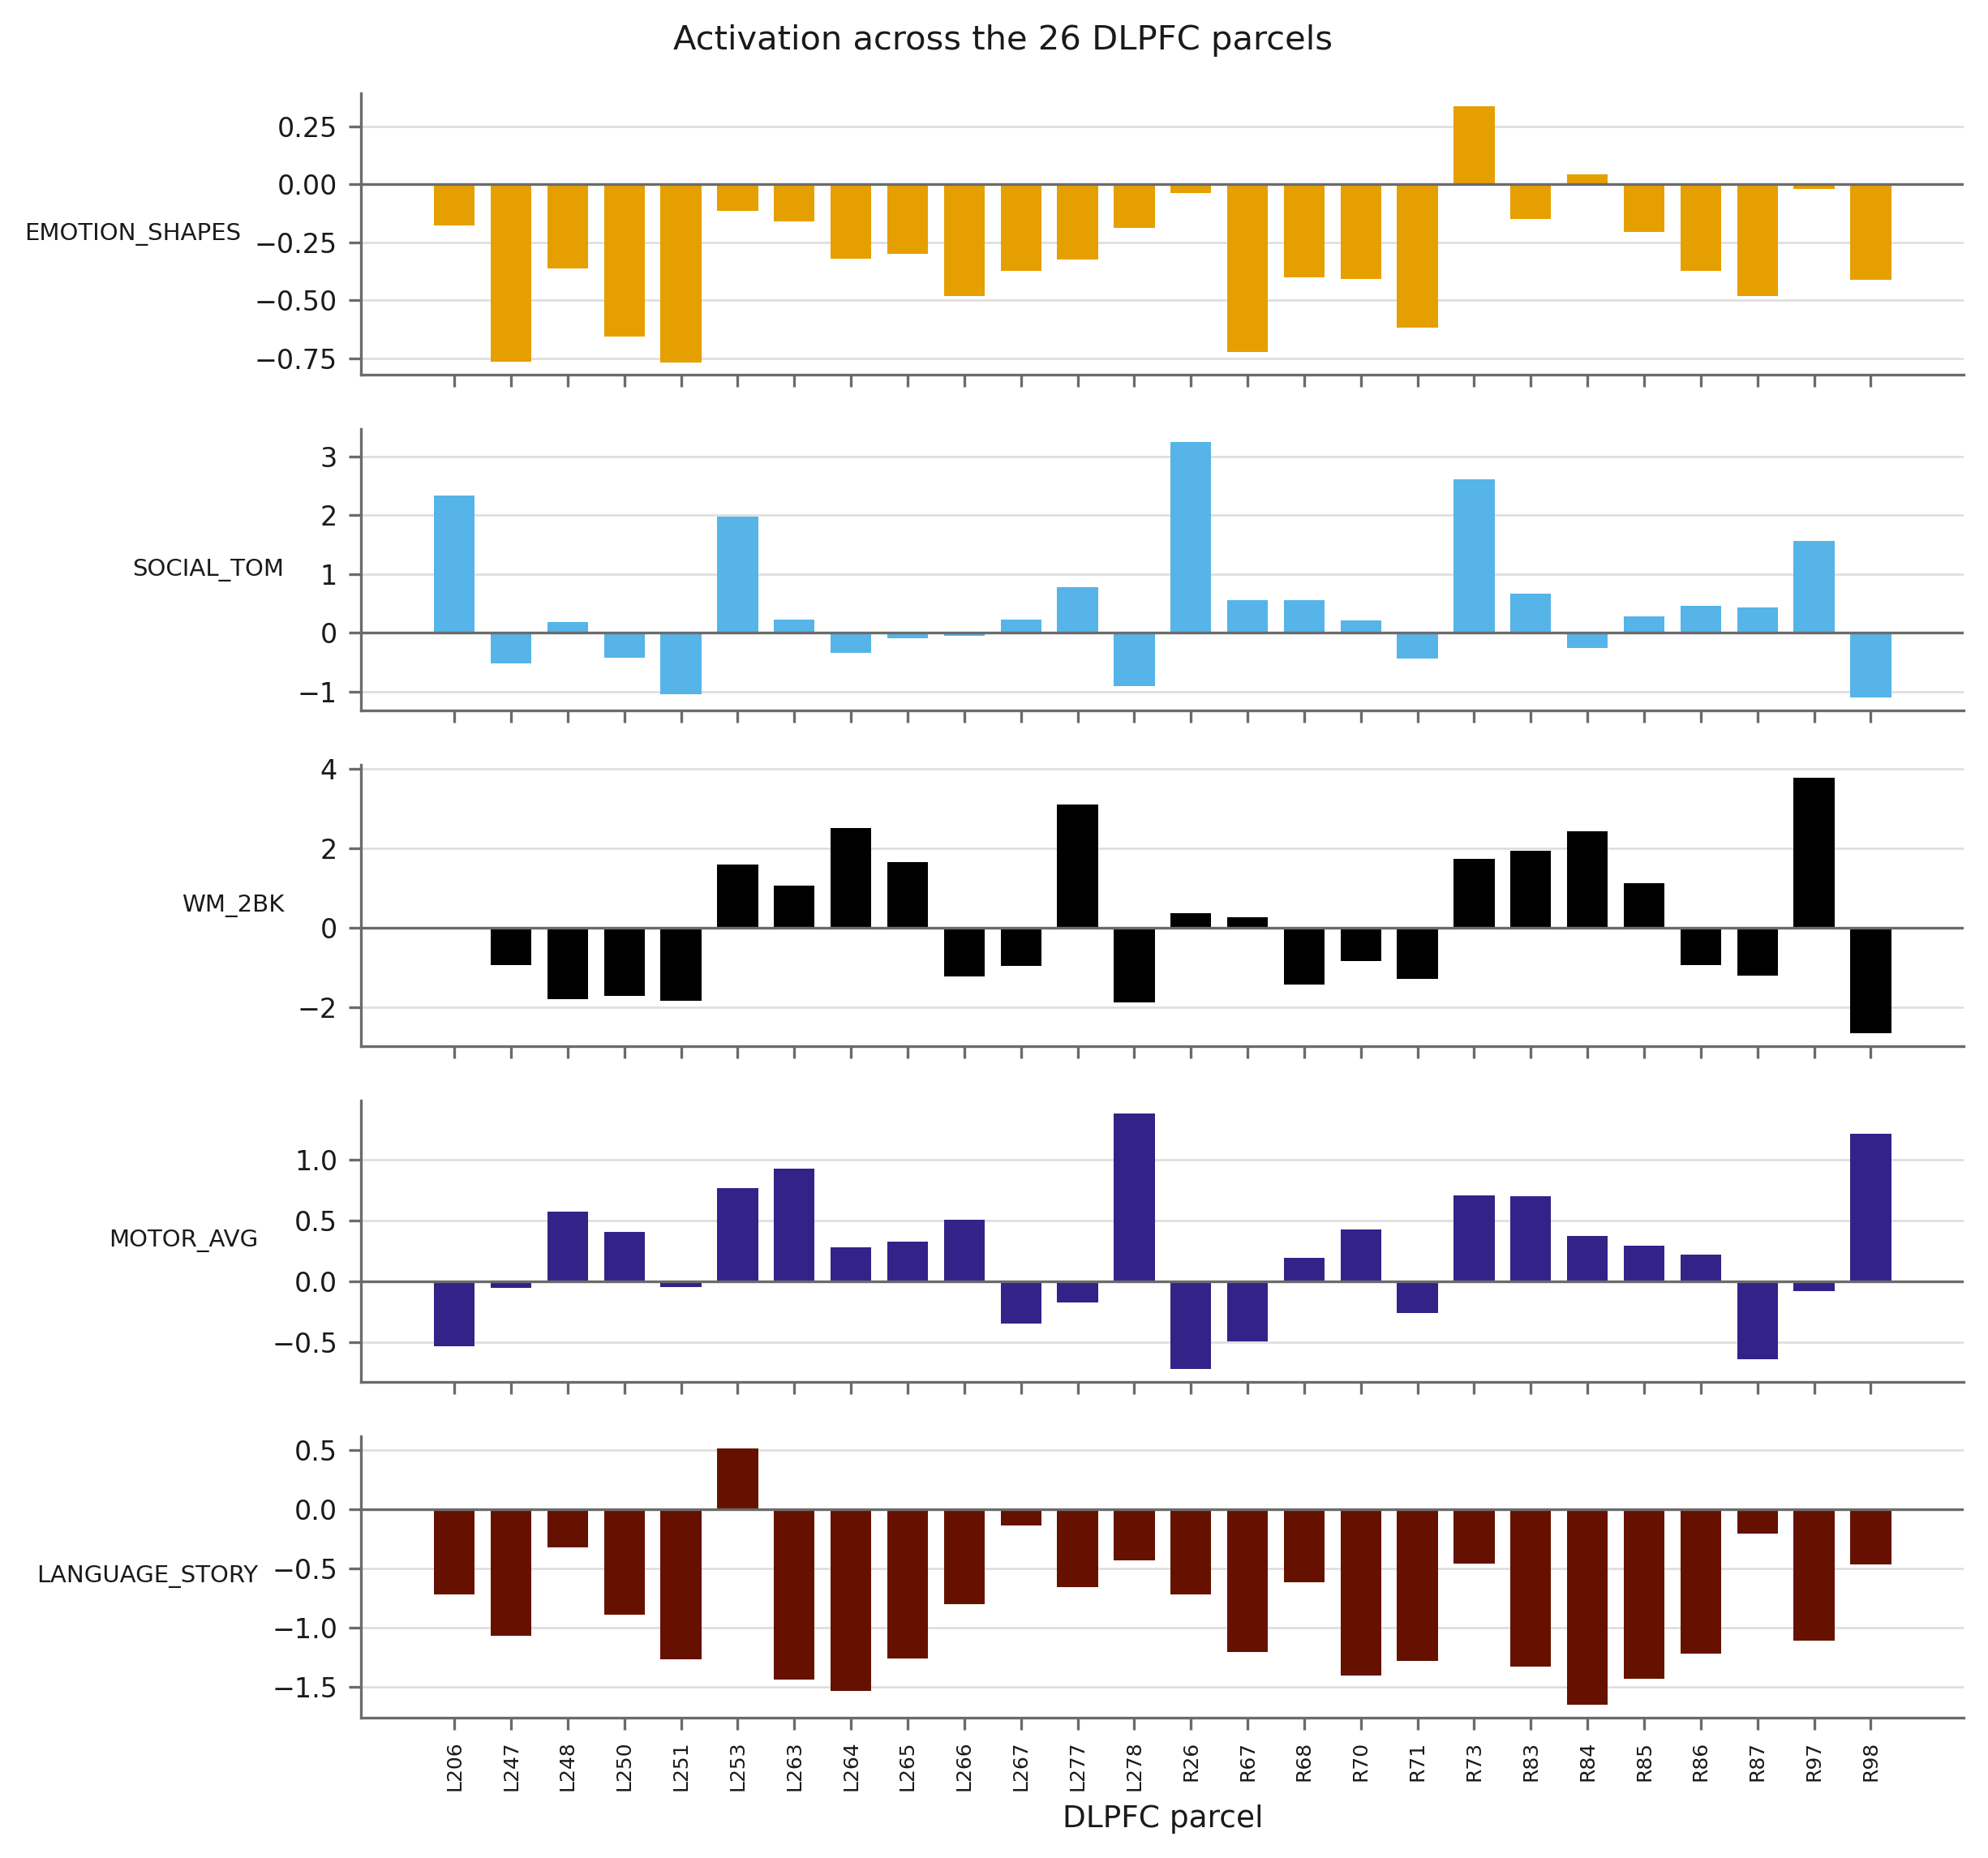
\includegraphics[width=.8\linewidth]{S5_parcel_profiles.png}
  \caption*{\textbf{Fig.~S5.} Activation profiles of the five representative
  contrasts across the 26 DLPFC parcels.}
\end{figure}

\begin{figure}[p]
  \centering
  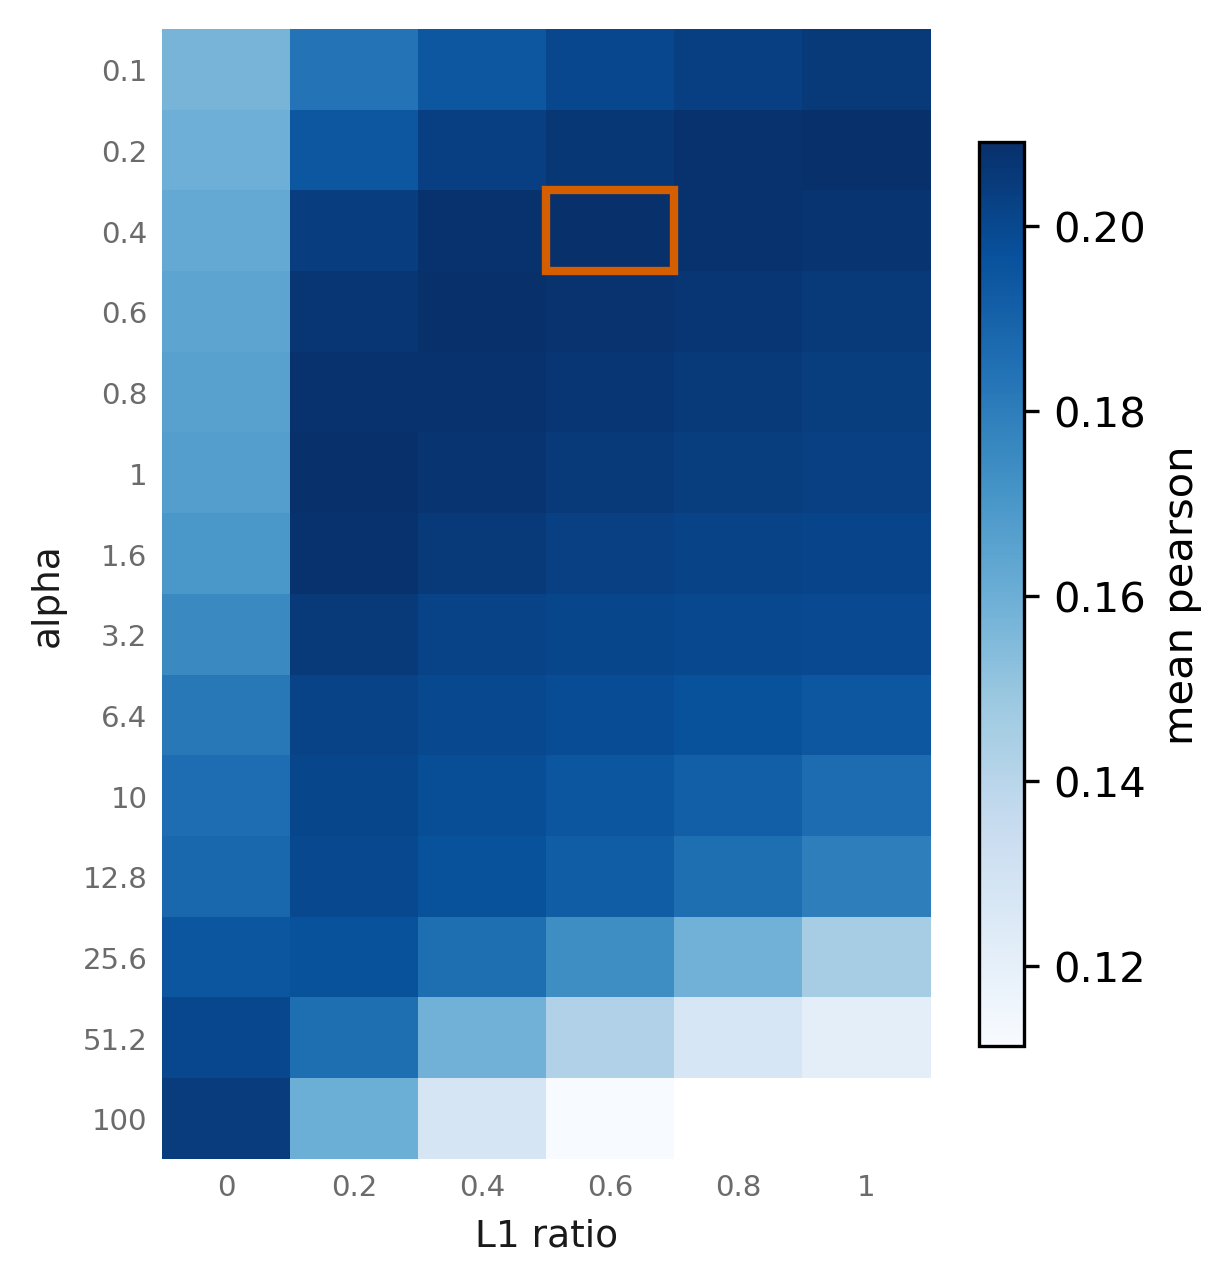
\includegraphics[width=.7\linewidth]{S6_hyperparameter_grid.png}
  \caption*{\textbf{Fig.~S6.} Hyperparameter grid on the 20 held-out tuning
  participants; the selected cell ($\alpha=0.4$, L1 ratio $=0.6$) ranks third
  of 84 by mean within-task correlation, 0.0001 from the grid maximum.}
\end{figure}

\begin{figure}[p]
  \centering
  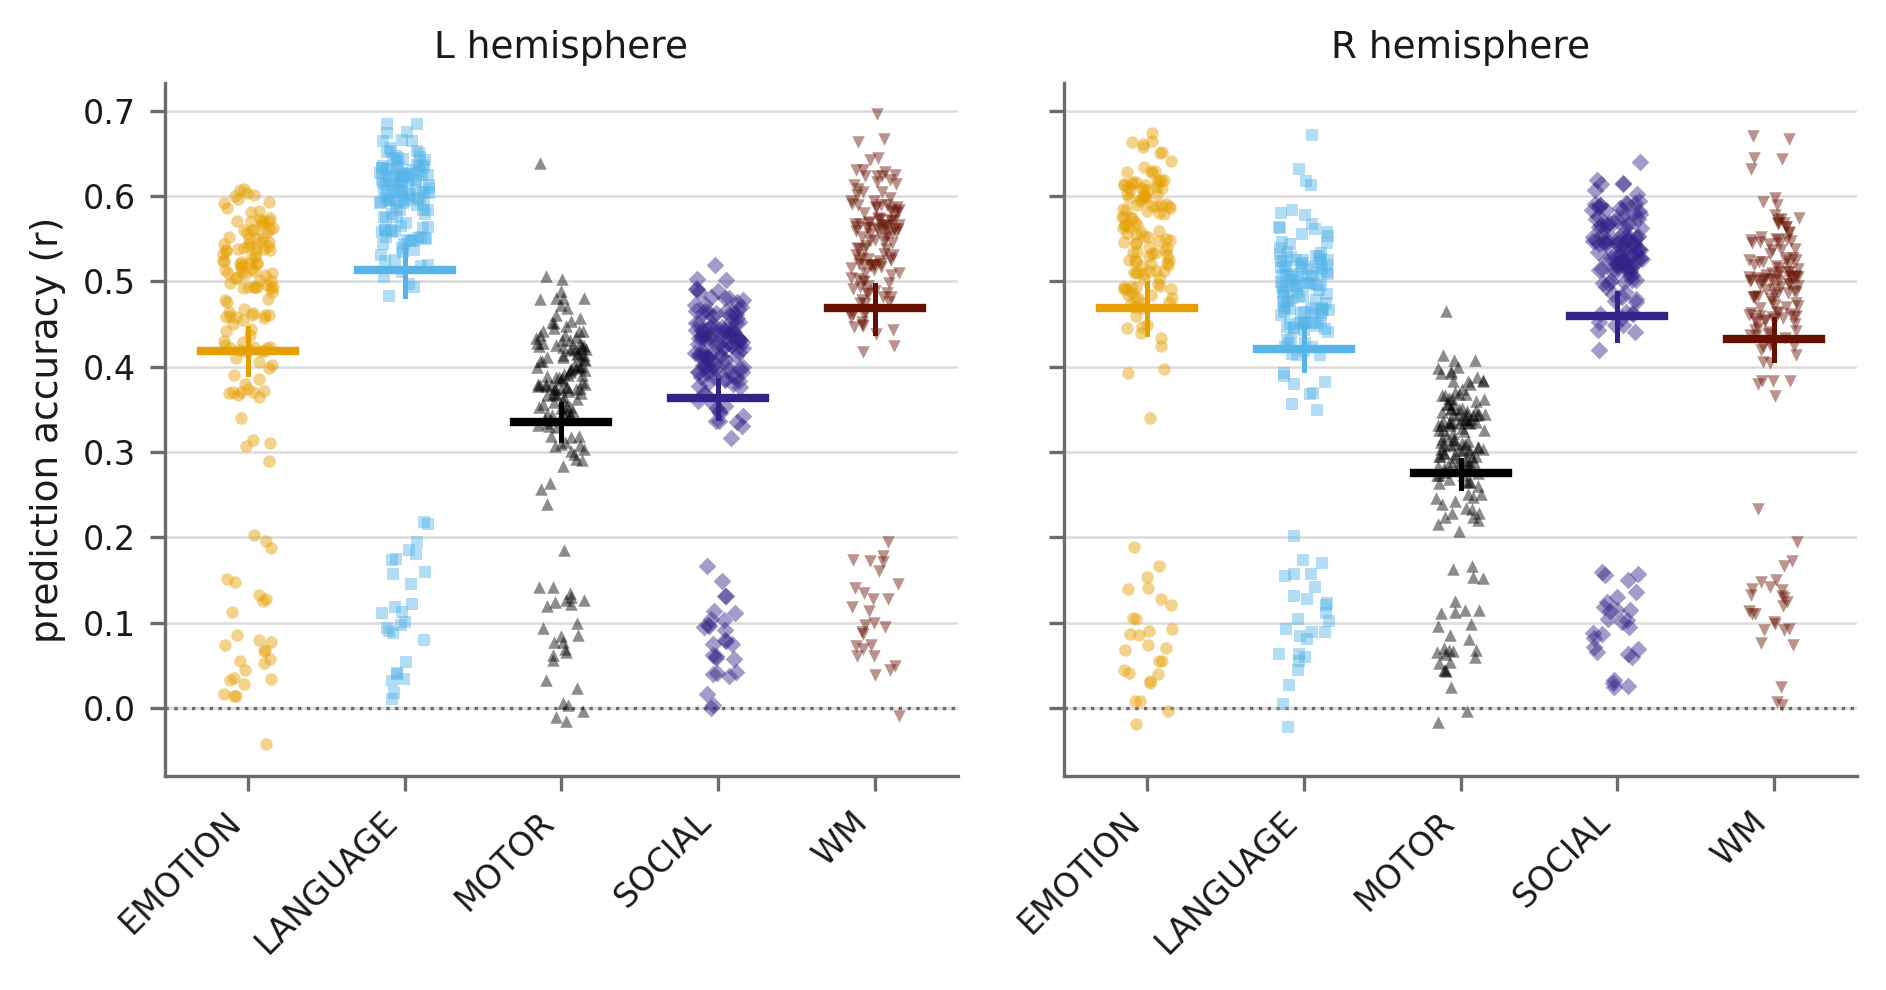
\includegraphics[width=.49\linewidth]{S7_adult_group_average_accuracy.png}
  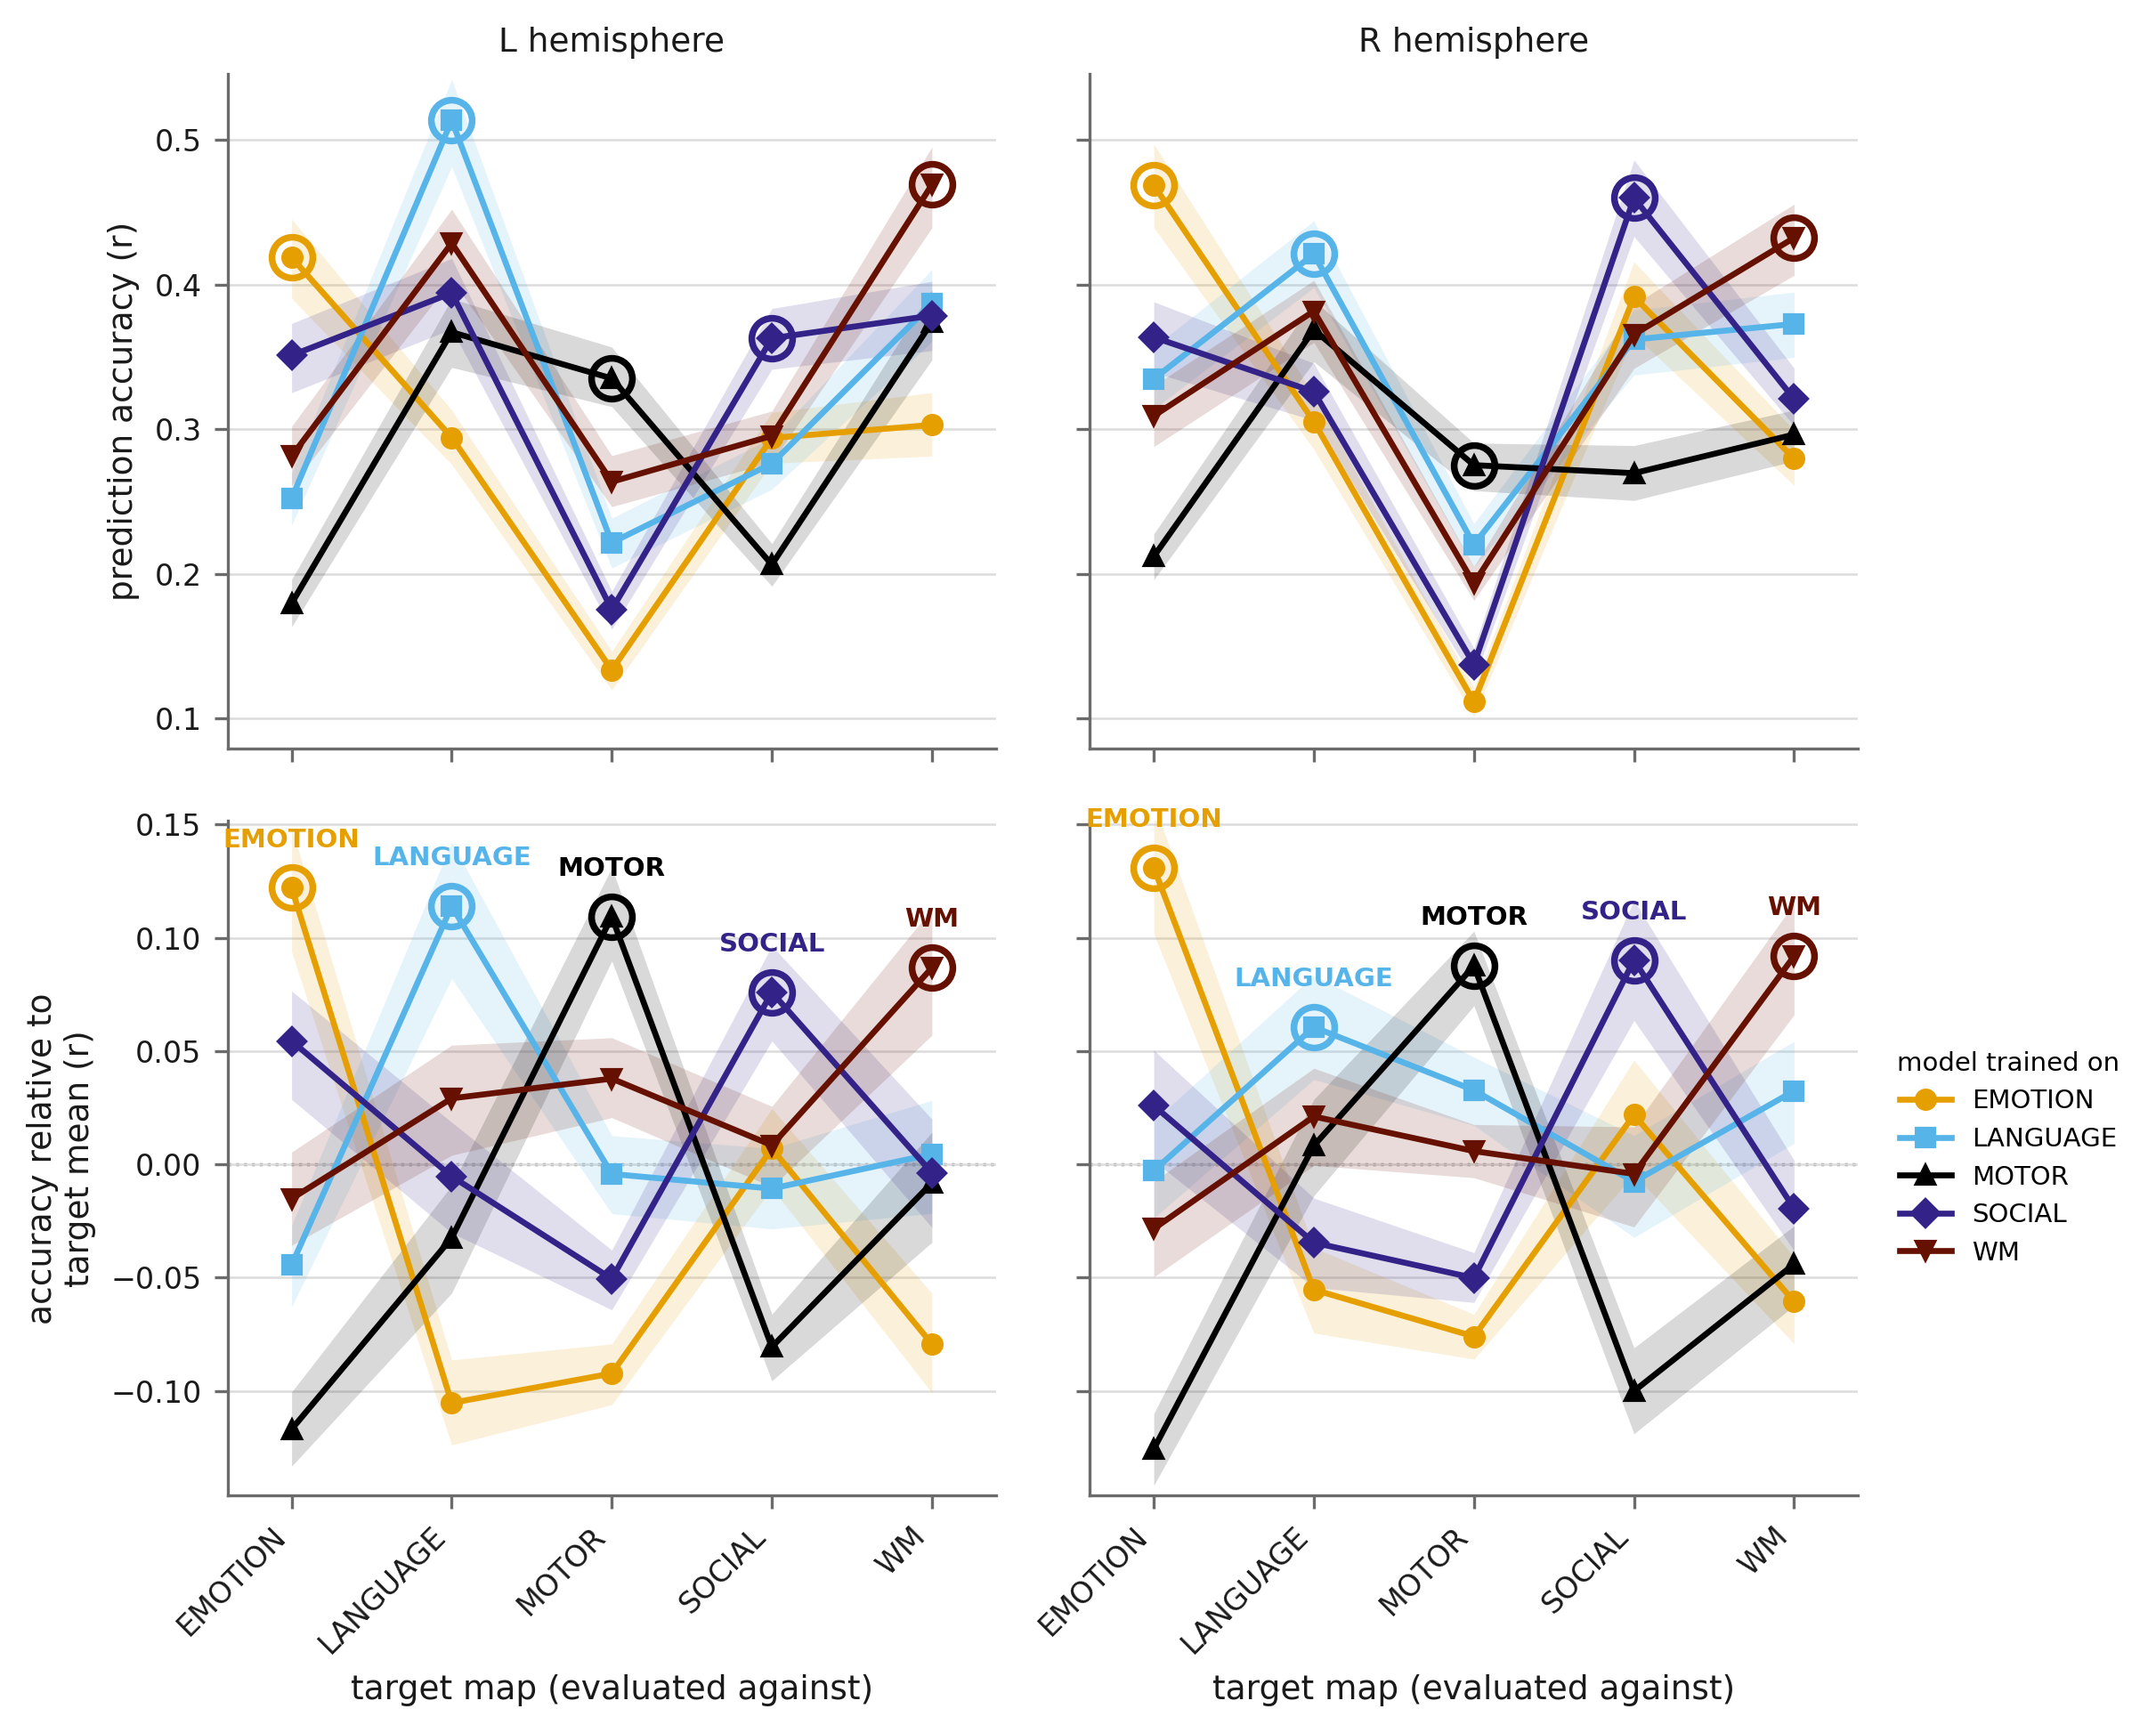
\includegraphics[width=.49\linewidth]{S7_adult_group_average_specificity.png}
  \caption*{\textbf{Fig.~S7.} Adult prediction of the group-average map
  (leave-one-participant-out): accuracy and task specificity.}
\end{figure}

\begin{figure}[p]
  \centering
  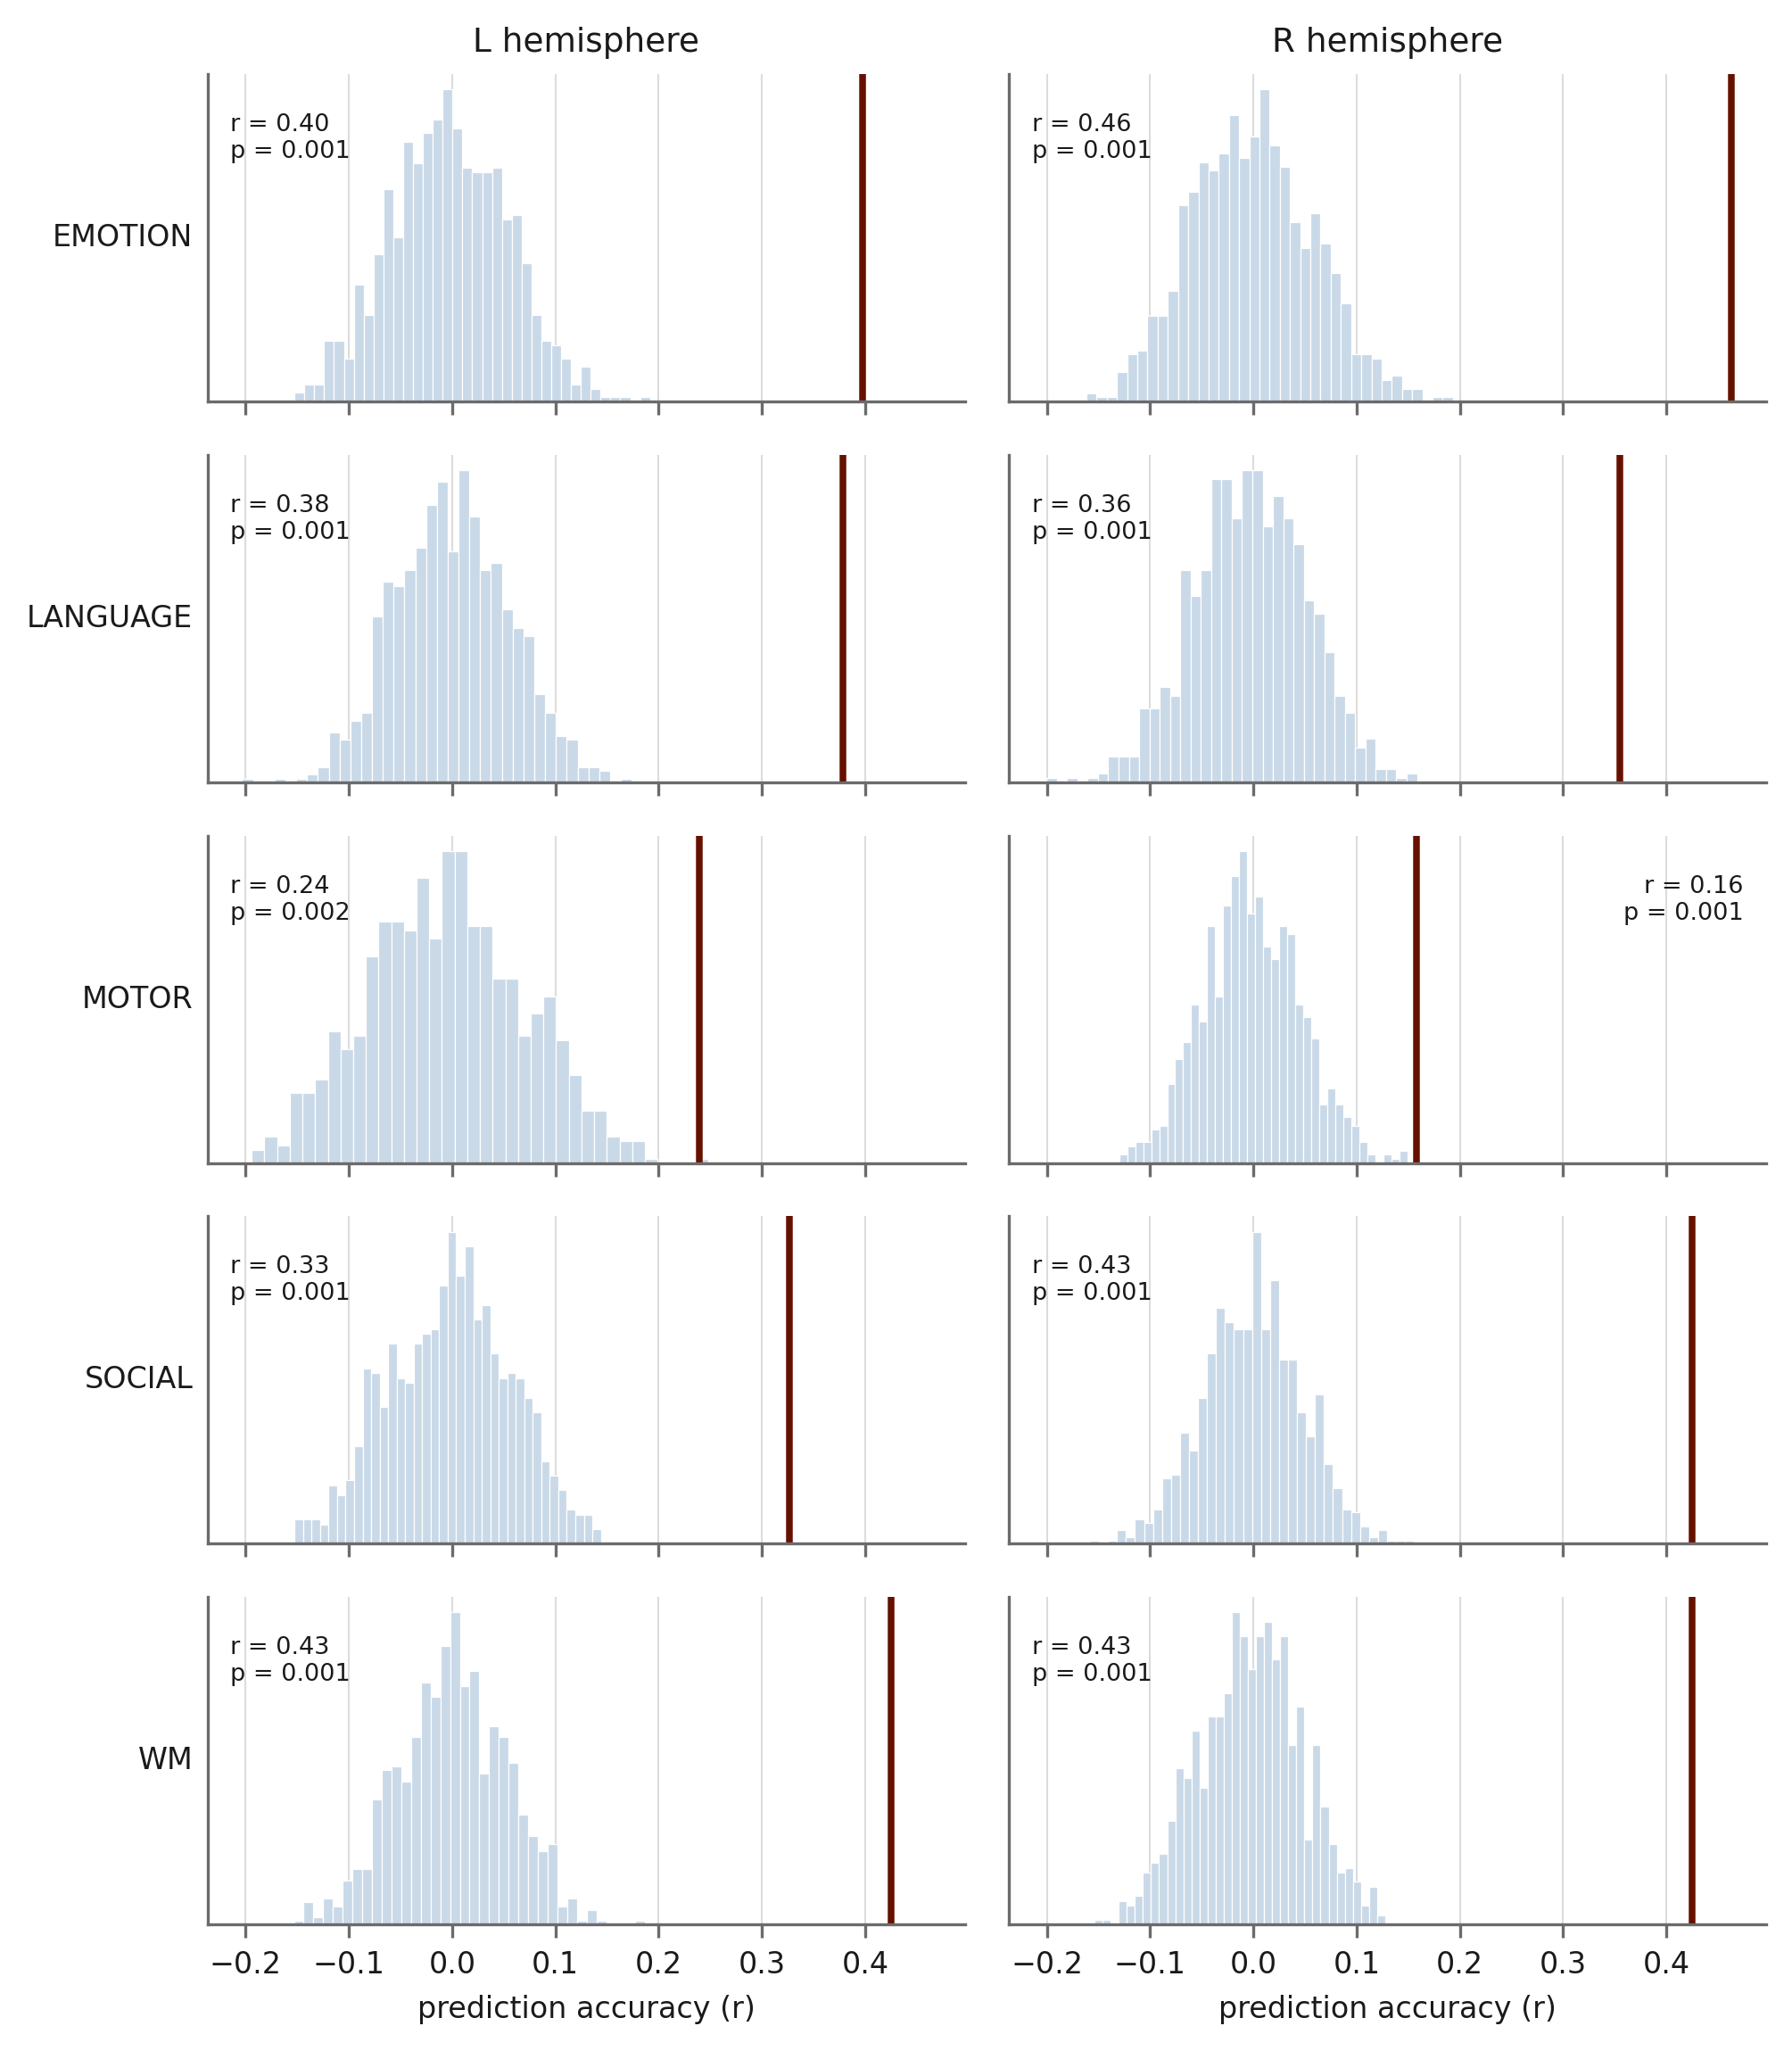
\includegraphics[width=.8\linewidth]{S8_spatial_null.png}
  \caption*{\textbf{Fig.~S8.} Output-level spatial null: observed
  across-neonate mean accuracy against 1{,}000 variogram-matched surrogates
  per contrast and hemisphere.}
\end{figure}

\begin{figure}[p]
  \centering
  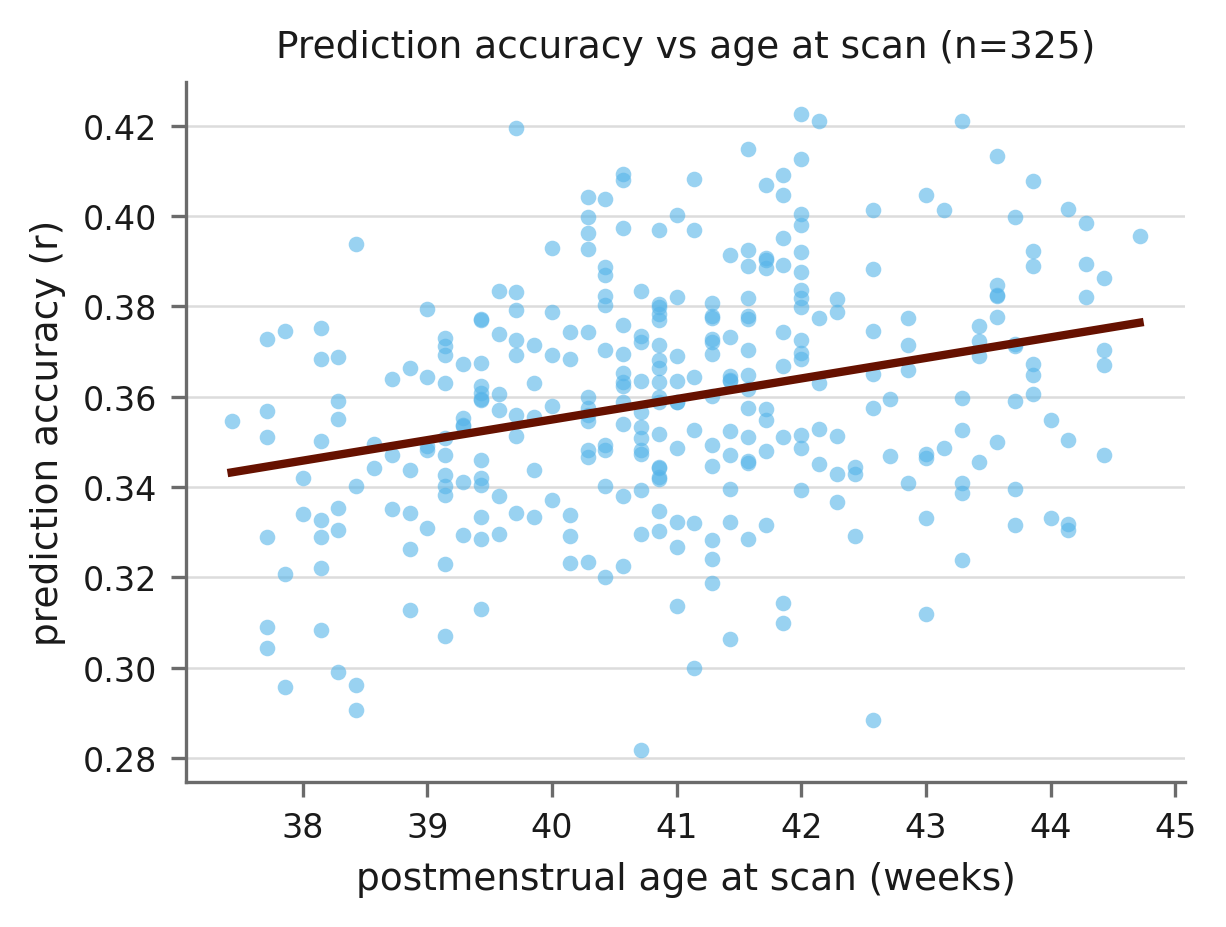
\includegraphics[width=.8\linewidth]{S9_scan_age.png}
  \caption*{\textbf{Fig.~S9.} Prediction accuracy against postmenstrual age
  at scan (exploratory; see Supplementary Methods).}
\end{figure}

\begin{figure}[p]
  \centering
  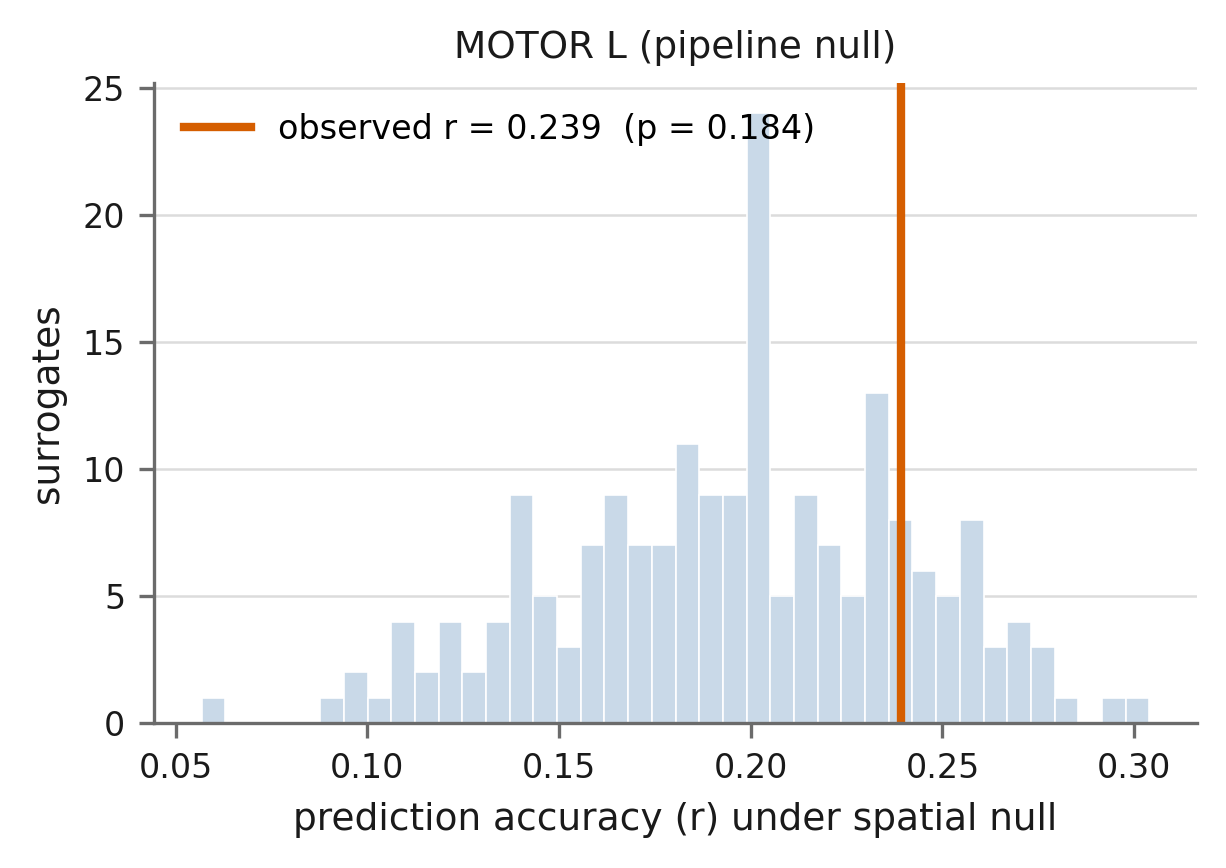
\includegraphics[width=.9\linewidth]{S10_pipeline_null_tfMRI_MOTOR_L.png}
  \caption*{\textbf{Fig.~S10.} Full-pipeline surrogate null, one panel per
  contrast and hemisphere (left motor shown; remaining panels in
  figures/manuscript/). [Assemble the 10-panel grid for submission.]}
\end{figure}

\section{Supplementary Tables}

\noindent\textbf{Table~S1.} The 13 DLPFC parcels per hemisphere of the HCP
multimodal parcellation (SFL, 8Av, 8Ad, 8BL, 9p, 8C, p9-46v, 46, a9-46v,
9-46d, 9a, i6-8, s6-8). [Generate the full table with
\texttt{pipelines/02\_rois/make\_table\_s1.py}.]

\bibliographystyle{plainnat}
\bibliography{references}

\end{document}
